\documentclass[11pt,a4paper]{article}

\usepackage[T1]{fontenc}
\usepackage[utf8]{inputenc}
\usepackage{lmodern}
\usepackage[margin=20mm]{geometry}
\usepackage{graphicx}
\usepackage{float}
\usepackage{booktabs}
\usepackage{longtable}
\usepackage{array}
\usepackage{amsmath}
\usepackage{xcolor}
\usepackage{hyperref}
\usepackage{tikz}
\usetikzlibrary{arrows.meta,positioning,shapes.geometric}

\hypersetup{
  colorlinks=true,
  linkcolor=blue!50!black,
  urlcolor=blue!50!black
}

\graphicspath{{figures/}}
\setlength{\parskip}{0.55em}
\setlength{\parindent}{0pt}
\renewcommand{\arraystretch}{1.18}

\definecolor{boxblue}{RGB}{224,239,255}
\definecolor{boxgreen}{RGB}{227,245,232}
\definecolor{boxorange}{RGB}{255,240,218}
\definecolor{boxgray}{RGB}{241,243,245}

\title{\textbf{Cycle-Jump Technique and Abaqus/UMAT Validation}}
\author{Pruthvi}
\date{18 May 2026}

\begin{document}
\maketitle

\begin{center}
\fbox{\parbox{0.92\linewidth}{
\textbf{Short message.}
This work develops and validates a cycle-jump workflow for a Chaboche-type viscoplastic UMAT in Abaqus. The method uses a few no-skip baseline cycles to predict a later material state, injects that state using \texttt{SDVINI} and \texttt{SIGINI}, and checks the result against no-skip reference simulations. The partial 4380-cycle work and the current Stage 14 2000-cycle blockwise work are excluded from the completed-results list.
}}
\end{center}

\tableofcontents
\newpage

\section{One-Page Summary}

Fatigue simulations are expensive because Abaqus normally solves every load increment in every cycle. A direct 1000-cycle simulation is much slower than a 20-cycle simulation. The purpose of cycle jumping is to skip cycles while preserving the important internal material history.

The completed workflow is:

\begin{enumerate}
  \item Run a no-skip Abaqus reference for a small number of cycles.
  \item Extract cycle-end stress, reaction force, and \texttt{STATEV} values.
  \item Identify a slow internal variable. Here the most important one is \texttt{STATEV1}, accumulated viscoplastic strain.
  \item Predict a future cycle state using the cycle-to-cycle increment.
  \item Re-initialize Abaqus at the predicted state using \texttt{SDVINI} for state variables and \texttt{SIGINI} for initial stress.
  \item Continue the simulation and compare it with a no-skip reference.
\end{enumerate}

The most important completed result is the Stage 12 1000-cycle percentage jump:

\begin{center}
\begin{tabular}{ll}
\toprule
Best accepted route & cycle 10 $\rightarrow$ predicted state at cycle 373 $\rightarrow$ continue to cycle 1000 \\
Skipped intermediate FE cycles & 362 \\
Final \texttt{STATEV1} error & 0.998969124476\% \\
Final S11 error & 0.114850661342\% \\
Final RF1 error & 0.114850661342\% \\
Decision & accepted clean success \\
\bottomrule
\end{tabular}
\end{center}

\section{Full-Run and Cycle-Jump Comparison}

The table below compares selected completed cycle-jump results with their corresponding full no-skip Abaqus reference values. The last column gives the relative error of the cycle-jump result with respect to the full-run result.

\begin{longtable}{p{0.18\linewidth}p{0.18\linewidth}p{0.20\linewidth}p{0.20\linewidth}p{0.14\linewidth}}
\toprule
Case & Quantity & Full run value & Cycle-jump value & Error \\
\midrule
\endhead
Cycle 20 & \texttt{STATEV1} & 0.142025694251 & 0.141955494881 & 0.049427\% \\
Cycle 20 & S11 [MPa] & 376.434143066 & 375.956024170 & 0.127013\% \\
Cycle 50 & \texttt{STATEV1} & 0.356620669365 & 0.357523173094 & 0.253071\% \\
Cycle 50 & S11 [MPa] & 374.653869629 & 374.458190918 & 0.052229\% \\
Cycle 50 & RF1 & 1498.61547852 & 1497.83276367 & 0.052229\% \\
Cycle 100 & \texttt{STATEV1} & 0.712048649788 & 0.716804206371 & 0.667870\% \\
Cycle 100 & S11 [MPa] & 371.760040283 & 372.025390625 & 0.071377\% \\
Cycle 100 & RF1 & 1487.04016113 & 1488.10156250 & 0.071377\% \\
Cycle 1000 & \texttt{STATEV1} & 6.70427989960 & 6.77125358582 & 0.998969\% \\
Cycle 1000 & S11 [MPa] & 330.549835205 & 330.170196533 & 0.114851\% \\
Cycle 1000 & RF1 & 1322.19934082 & 1320.68078613 & 0.114851\% \\
\bottomrule
\end{longtable}

The conclusion from the comparison is that the cycle-jump method reproduced the full-run accumulated state with less than 1\% error for the accepted cases. Stress and reaction force errors were generally much smaller than the \texttt{STATEV1} error. Therefore, \texttt{STATEV1} is the controlling accuracy measure.

\section{Cycle-Jump Workflow Chart}

\begin{figure}[h!]
\centering
\resizebox{0.98\linewidth}{!}{
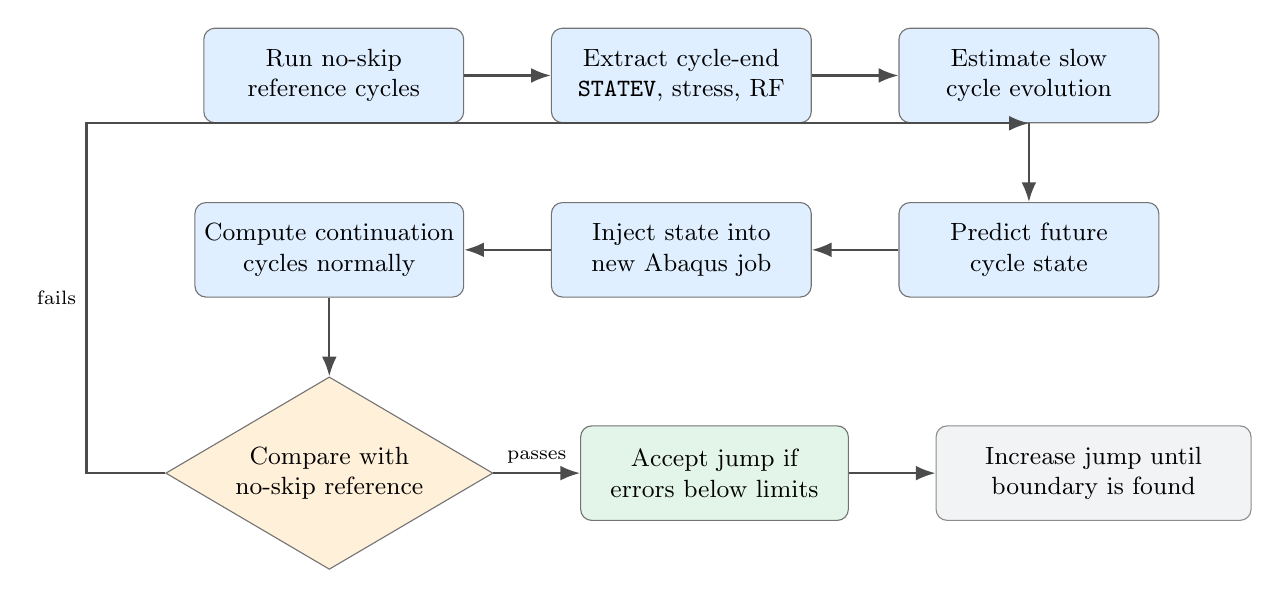
\begin{tikzpicture}[
  node distance=10mm and 11mm,
  cjblock/.style={rectangle, rounded corners, draw=black!55, fill=boxblue, minimum width=33mm, minimum height=12mm, align=center, font=\small},
  check/.style={diamond, aspect=1.7, draw=black!55, fill=boxorange, minimum width=31mm, align=center, font=\small},
  cjout/.style={rectangle, rounded corners, draw=black!55, fill=boxgreen, minimum width=34mm, minimum height=12mm, align=center, font=\small},
  note/.style={rectangle, rounded corners, draw=black!45, fill=boxgray, minimum width=40mm, minimum height=12mm, align=center, font=\small},
  arr/.style={-{Latex[length=2.5mm]}, thick, draw=black!70}
]
\node[cjblock] (run) {Run no-skip\\reference cycles};
\node[cjblock, right=of run] (extract) {Extract cycle-end\\\texttt{STATEV}, stress, RF};
\node[cjblock, right=of extract] (slope) {Estimate slow\\cycle evolution};
\node[cjblock, below=of slope] (predict) {Predict future\\cycle state};
\node[cjblock, left=of predict] (inject) {Inject state into\\new Abaqus job};
\node[cjblock, left=of inject] (continue) {Compute continuation\\cycles normally};
\node[check, below=of continue] (verify) {Compare with\\no-skip reference};
\node[cjout, right=of verify] (accept) {Accept jump if\\errors below limits};
\node[note, right=of accept] (limit) {Increase jump until\\boundary is found};

\draw[arr] (run) -- (extract);
\draw[arr] (extract) -- (slope);
\draw[arr] (slope) -- (predict);
\draw[arr] (predict) -- (inject);
\draw[arr] (inject) -- (continue);
\draw[arr] (continue) -- (verify);
\draw[arr] (verify) -- node[above, font=\scriptsize]{passes} (accept);
\draw[arr] (accept) -- (limit);
\draw[arr] (verify.west) -- ++(-1.0,0) |- node[pos=0.25, left, font=\scriptsize]{fails} (slope.south);
\end{tikzpicture}
}
\caption{Cycle-jump workflow used in this study. The loop is important: the jump size is increased only after the previous jump is verified against a no-skip reference.}
\end{figure}

\section{Theory in Simple Terms}

A cyclic inelastic material has memory. In the UMAT, that memory is stored in \texttt{STATEV}. If the material is loaded for many cycles, the stress oscillates quickly inside each cycle, but some internal variables evolve slowly from cycle to cycle.

Let $q_N$ be a selected state variable at the end of cycle $N$. The simplest cycle-jump estimate is:

\[
q_{N+\Delta N}^{pred}
= q_N + \Delta N \left\langle \frac{\Delta q}{\Delta N} \right\rangle
\]

In this project, the first successful predictor used:

\[
\texttt{STATEV1}_{pred}(N)
= \texttt{STATEV1}_{10}
+ (N-10)\,\overline{\Delta \texttt{STATEV1}}_{2-10}
\]

where \texttt{STATEV1} is accumulated viscoplastic strain. This is a physically meaningful variable because it increases monotonically and measures irreversible material history.

The slope used in this report is the mean of cycle-by-cycle increments, not one large secant line drawn only between cycle 2 and cycle 10:
\[
\overline{\Delta Q}_{2-10}
=
\frac{1}{9}
\sum_{i=2}^{10}
\left(Q_i-Q_{i-1}\right).
\]
The prediction from cycle 10 to a later cycle $N$ is then
\[
Q_N^{\mathrm{pred}}
=
Q_{10}
+
(N-10)\overline{\Delta Q}_{2-10}.
\]
Thus, the workflow computes the increment for each complete cycle and then averages the increments from cycles 2--10. This wording is important because it avoids confusing the method with a single coarse secant slope between only two points.

\section{Visual Walkthrough of the Work}

\subsection{Model and Boundary Conditions}

\begin{figure}[h!]
\centering
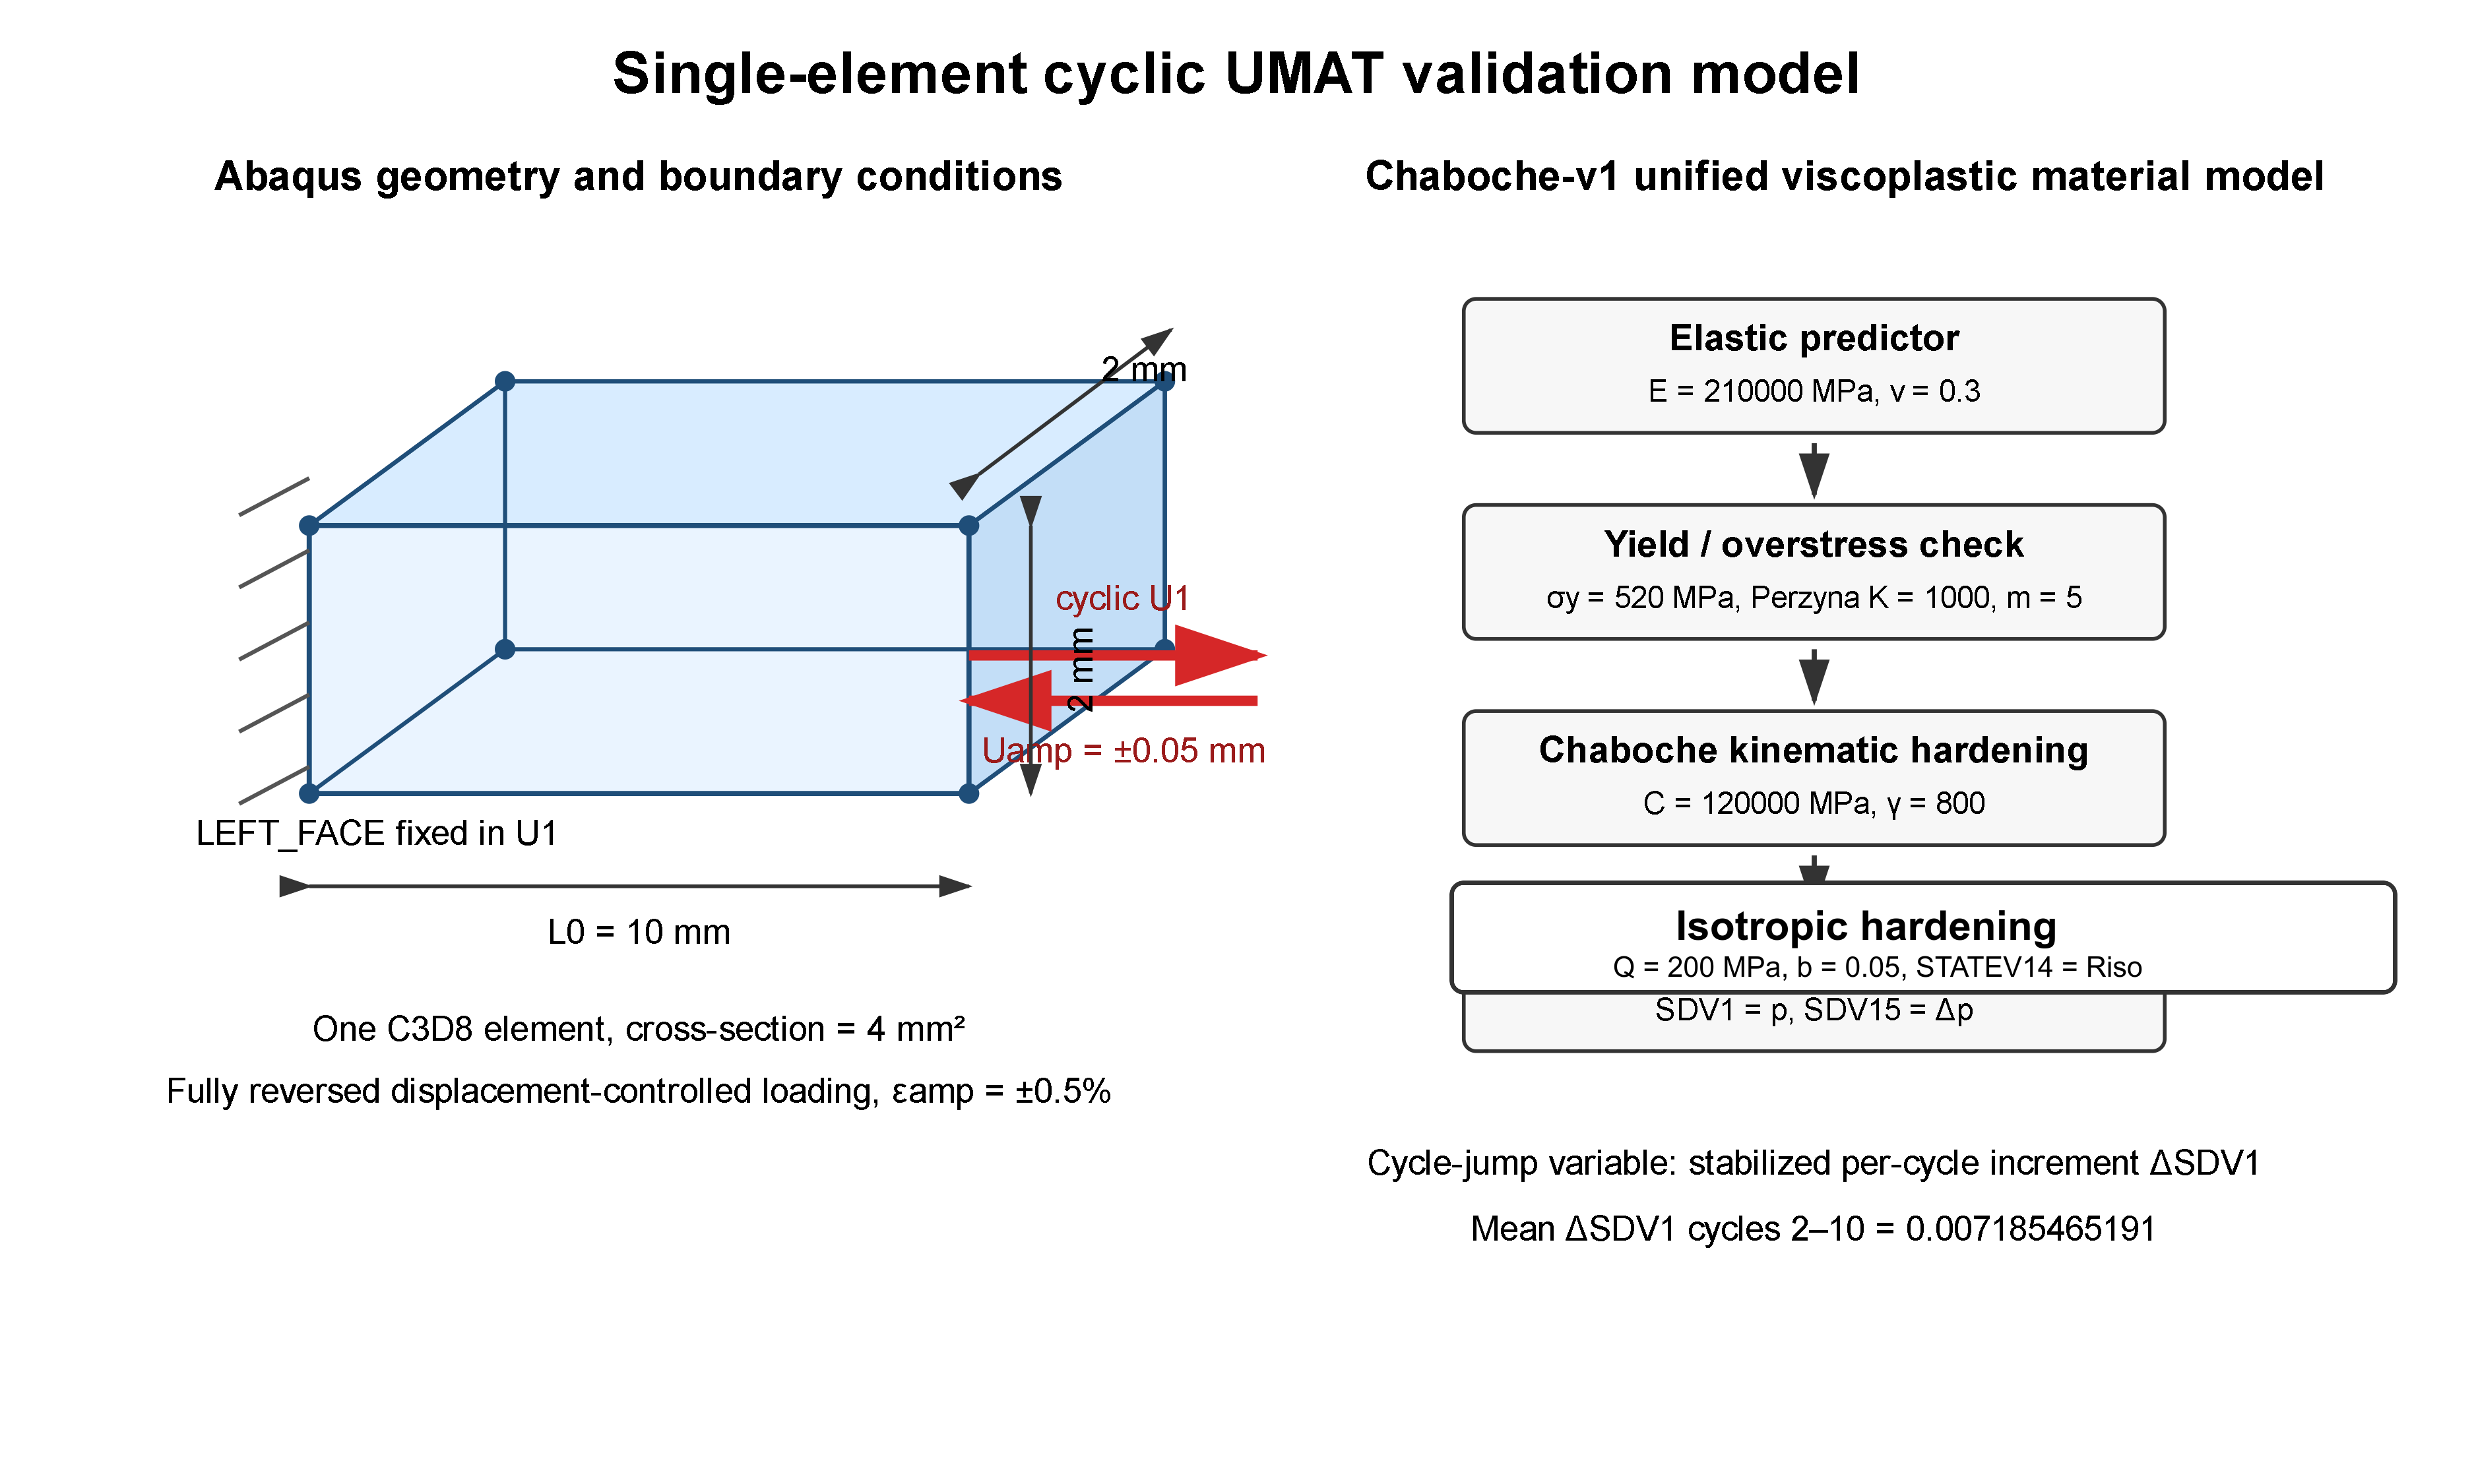
\includegraphics[width=0.82\linewidth]{fig00_geometry_material_model.png}
\caption{Simple single-element model used to validate the UMAT and cycle-jump idea. A simple model is useful because the internal state can be checked cleanly before moving to complex structures.}
\end{figure}

\begin{figure}[h!]
\centering
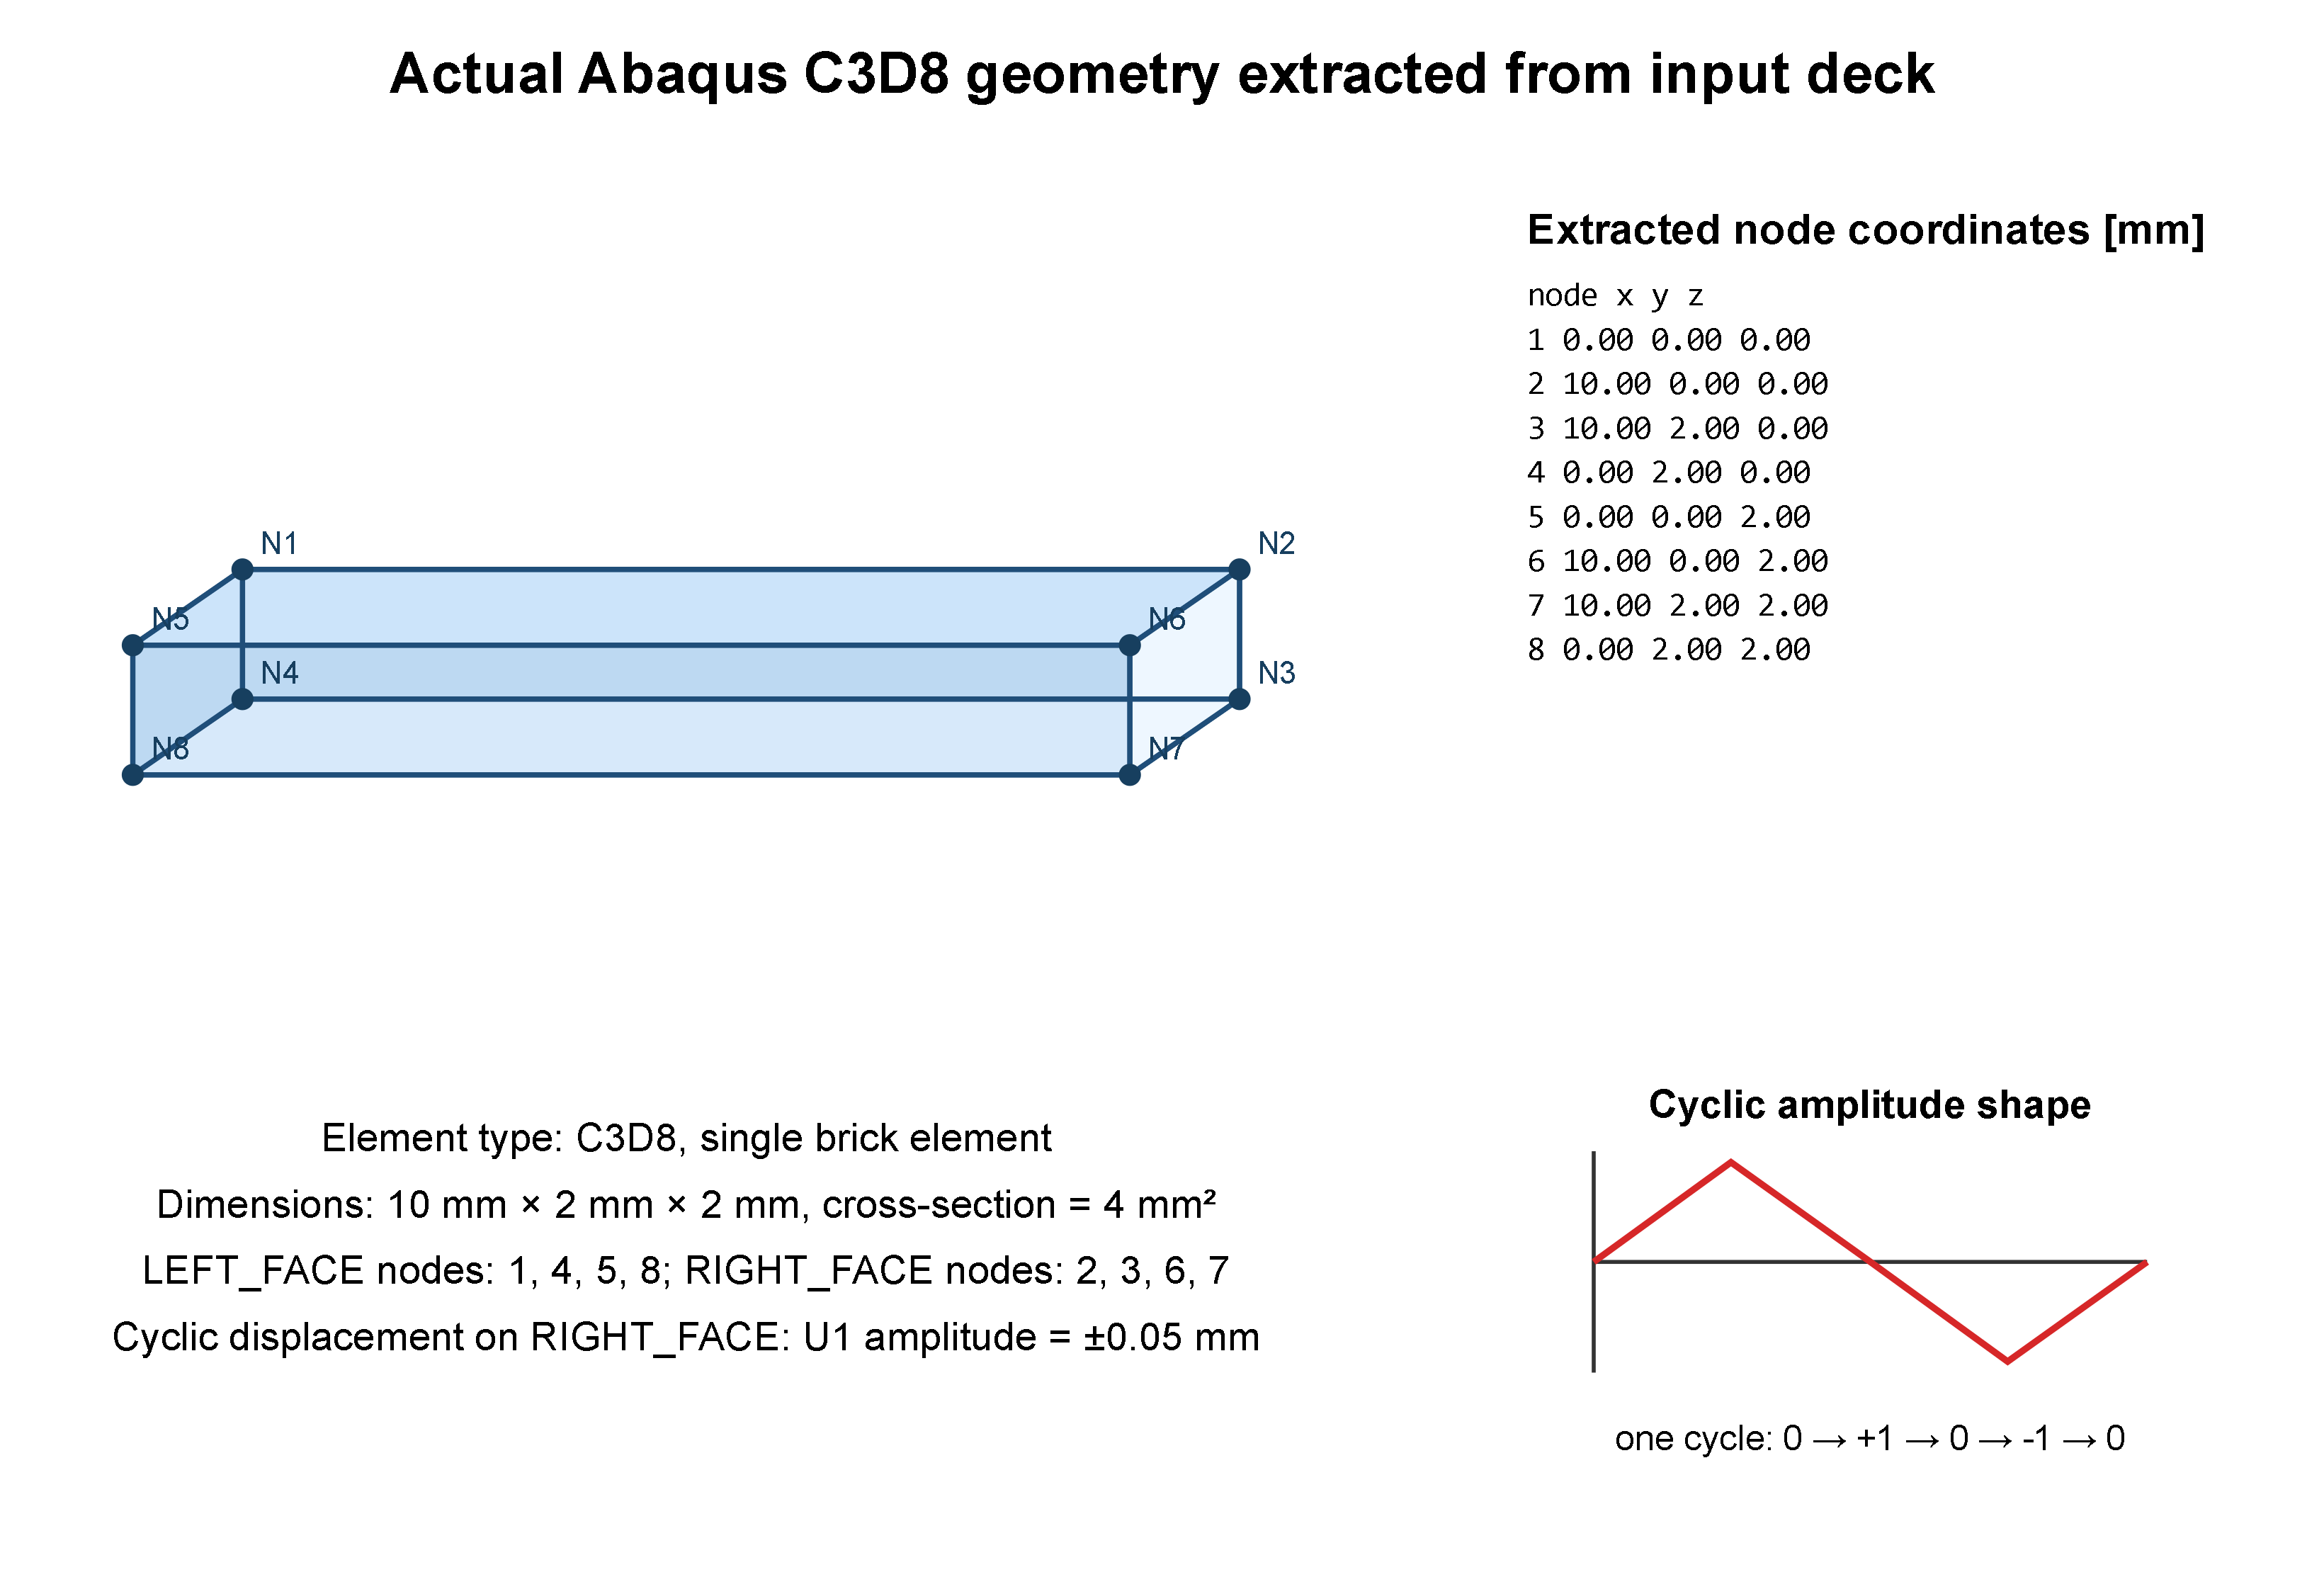
\includegraphics[width=0.82\linewidth]{fig00b_actual_abaqus_geometry.png}
\caption{Actual Abaqus geometry/output view used for the validation problem. The prescribed displacement controls the loading phase, while \texttt{STATEV} and stress carry the material history.}
\end{figure}

\subsection{Material Response Under Cyclic Loading}

\begin{figure}[h!]
\centering
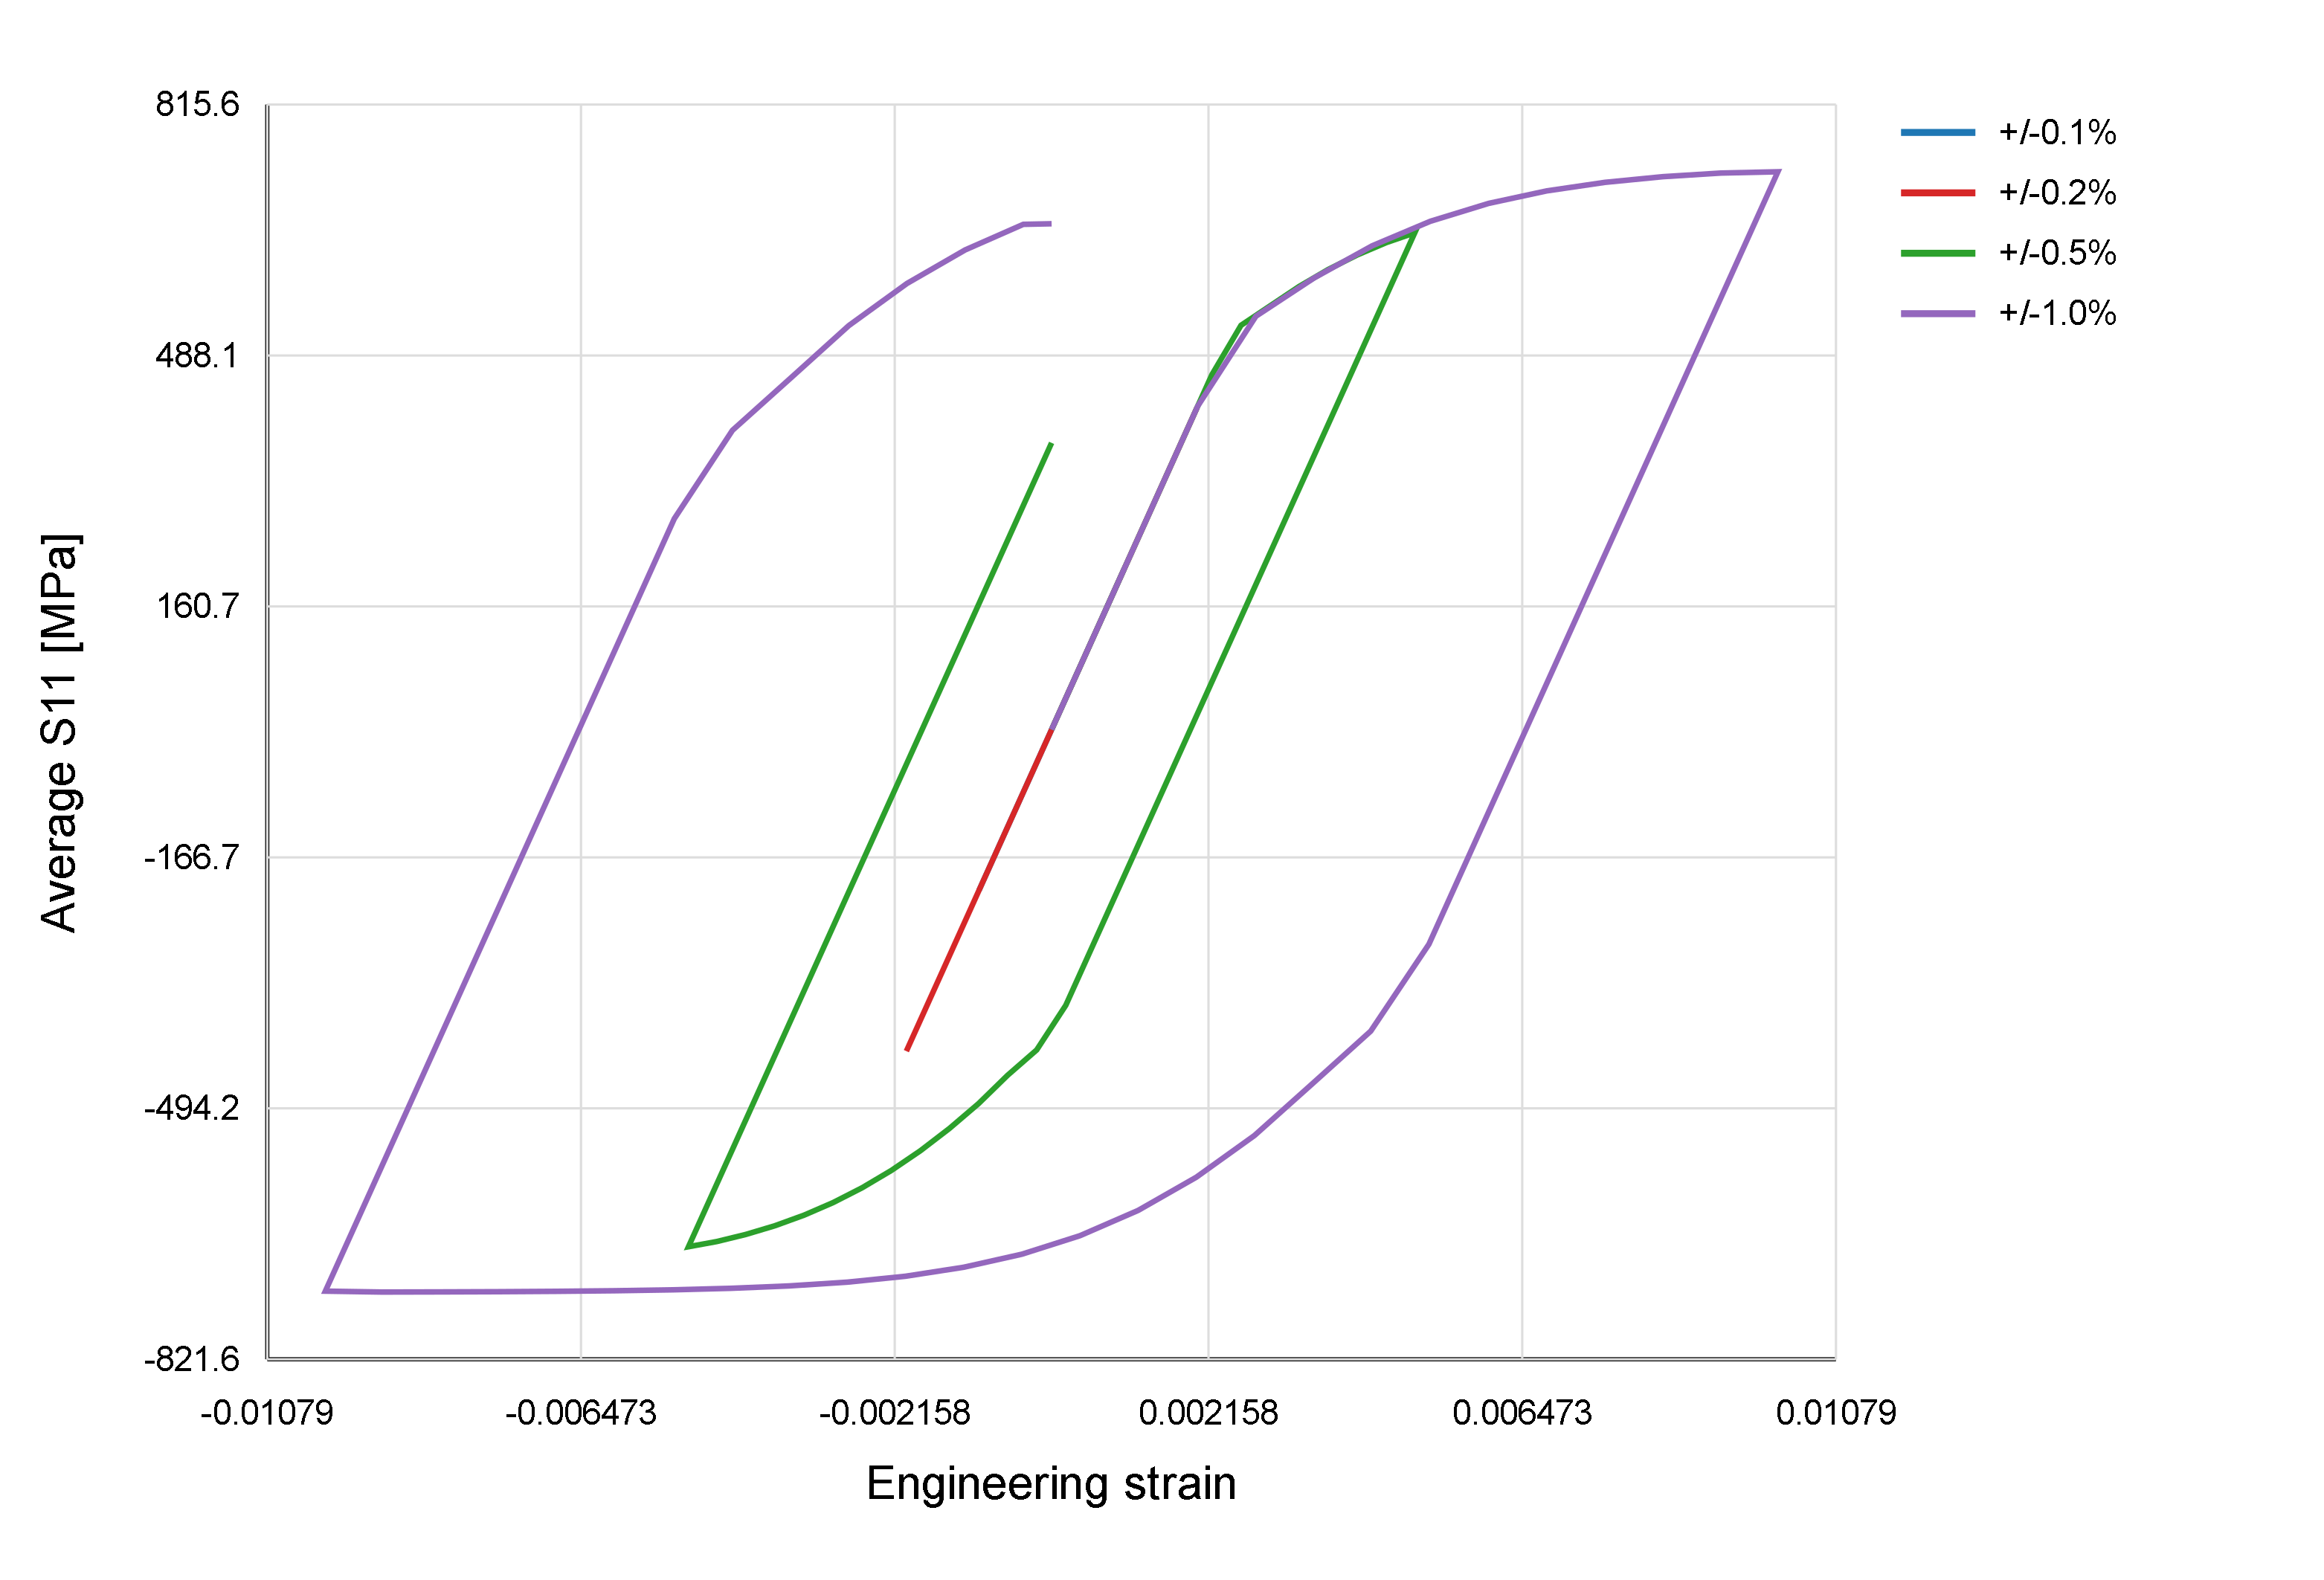
\includegraphics[width=0.82\linewidth]{fig01_amplitude_sweep_stress_strain.png}
\caption{Amplitude sweep for the Chaboche UMAT. Each colored line is a different imposed strain amplitude: for example, $\pm 0.1\%$ means the specimen is cycled between $-0.1\%$ and $+0.1\%$ engineering strain; $\pm 0.5\%$ means a larger cyclic strain range. The figure checks that the UMAT produces reasonable cyclic stress-strain loops before using it for cycle jumping.}
\end{figure}

\textbf{Explanation of Figure 4.}
The horizontal axis is strain and the vertical axis is stress. The colored curves correspond to different cyclic strain amplitudes. A larger strain amplitude gives a wider hysteresis loop and a larger stress range. This is expected for an inelastic Chaboche material: more severe cyclic loading creates more plastic or viscoplastic deformation. The conclusion is that the UMAT responds consistently over several loading amplitudes, so the $\pm 0.5\%$ case can be selected as the main validation amplitude for the cycle-jump study.

\clearpage

\begin{figure}[H]
\centering
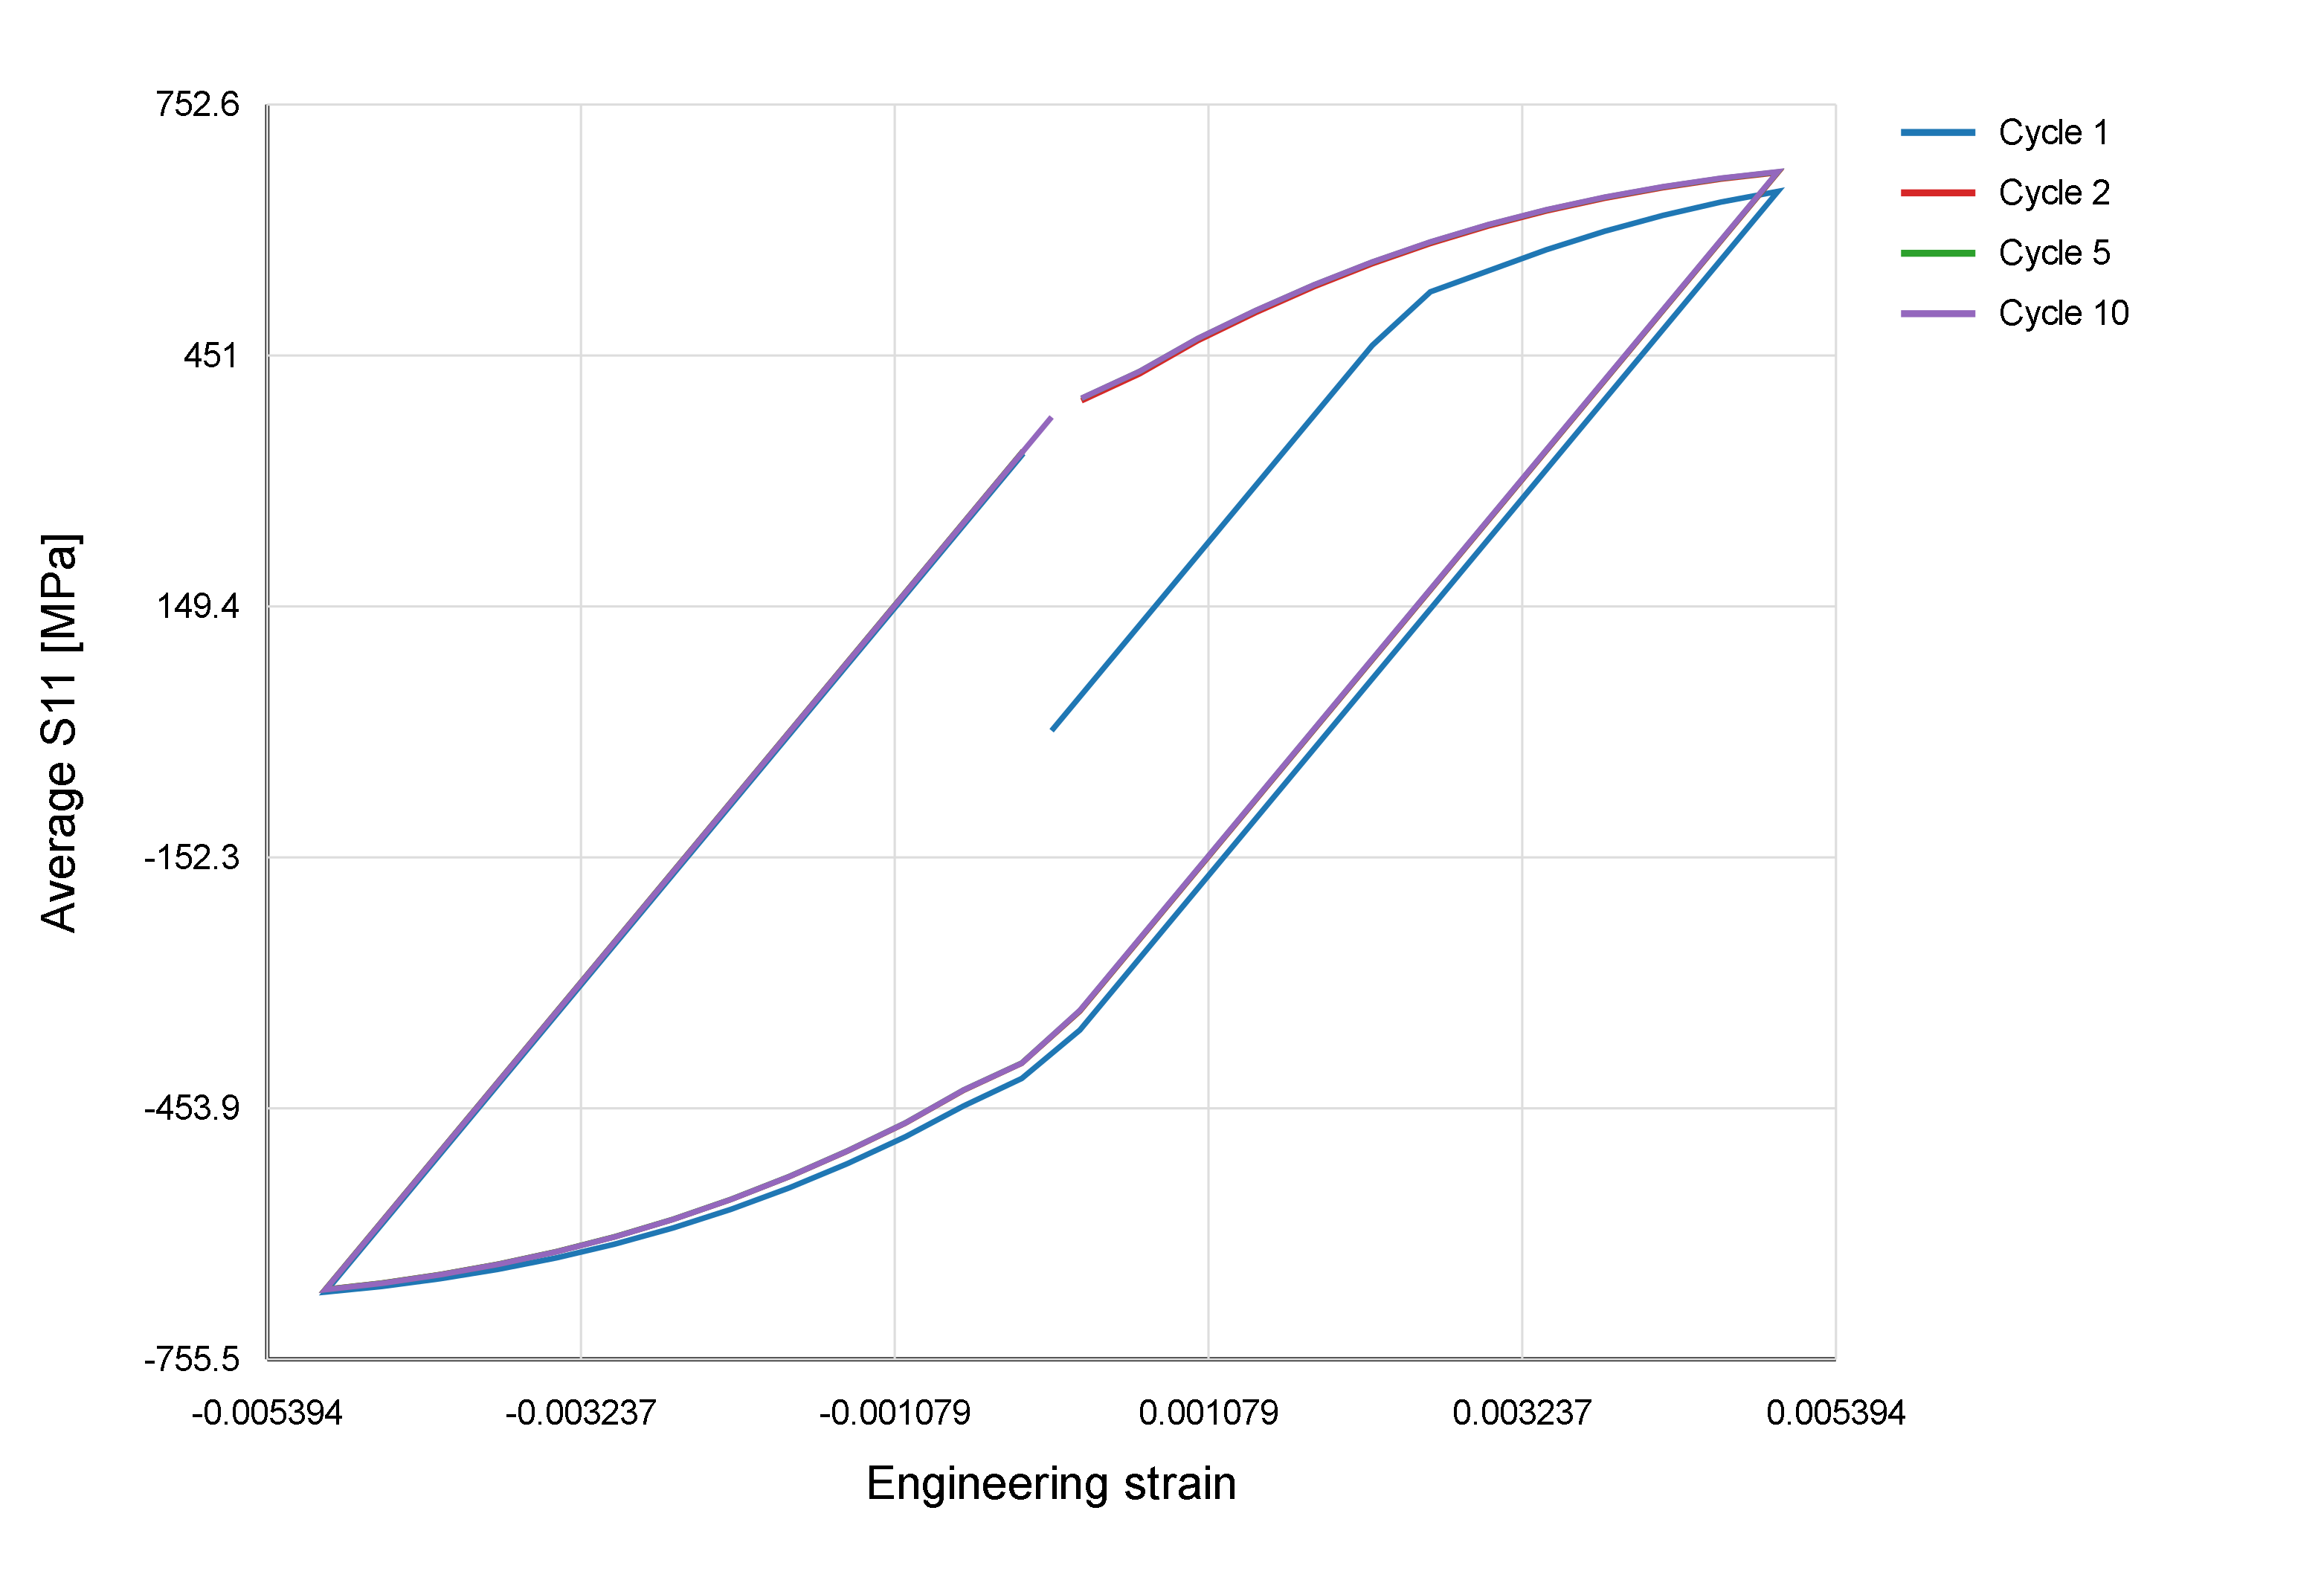
\includegraphics[width=0.82\linewidth]{fig02_10cycle_selected_hysteresis_loops.png}
\caption{Selected hysteresis loops from the 10-cycle baseline at the selected $\pm 0.5\%$ strain amplitude. Each line is one cycle or selected cycle from the no-skip Abaqus/Standard run.}
\end{figure}

\textbf{Explanation of Figure 5.}
This figure shows selected stress-strain hysteresis loops from the no-skip 10-cycle Abaqus/Standard baseline. The blue line is cycle 1, the red line is cycle 2, the green line is cycle 5, and the purple line is cycle 10. Some curves nearly overlap, especially the later cycles, which is why not every color is equally visible everywhere. Each loop is one complete loading and unloading cycle. If the loop shape keeps changing strongly, the material is still evolving rapidly. If later loops become similar, the cycle-to-cycle evolution is slower. The conclusion is that after the first cycles, the cyclic response is regular enough to search for a slowly evolving internal variable for cycle jumping.

\clearpage

\subsection{Finding a Slow Variable for Cycle Jumping}

\begin{figure}[H]
\centering
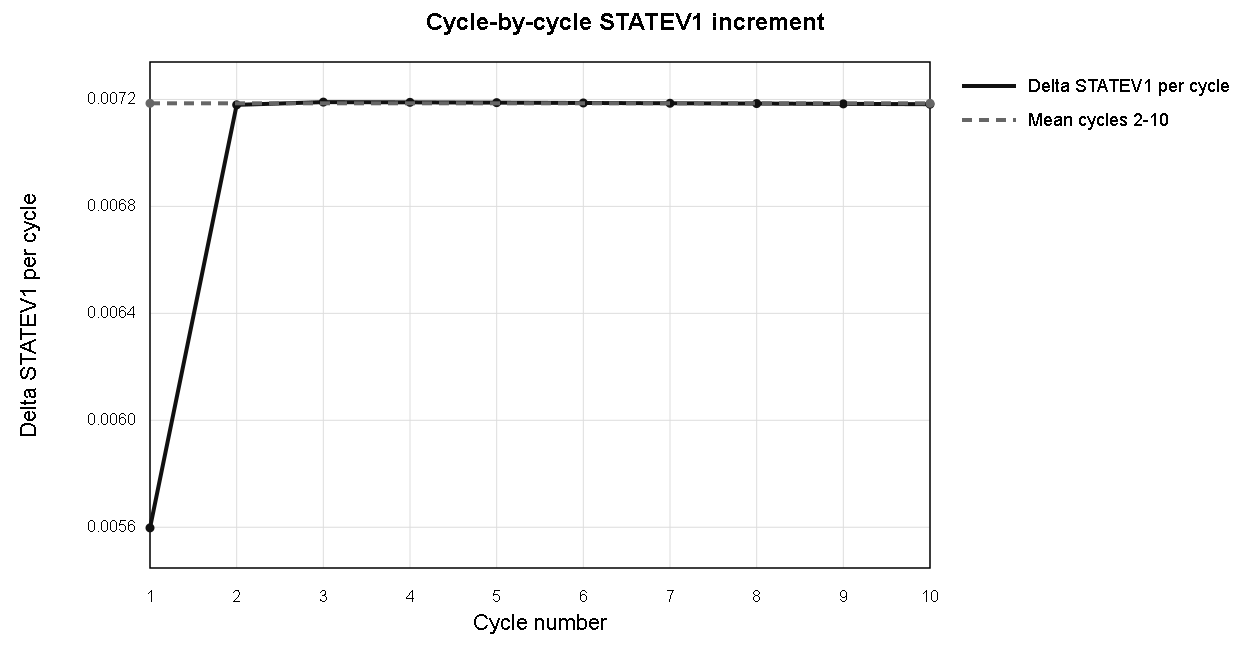
\includegraphics[width=0.80\linewidth]{fig03_delta_sdv1_per_cycle.png}
\caption{Cycle-by-cycle increment of \texttt{STATEV1}. Here \texttt{STATEV1} is accumulated viscoplastic strain, and $\Delta\texttt{STATEV1}$ is how much it increases during one cycle.}
\end{figure}

\textbf{Explanation of Figure 6.}
The horizontal axis is the integer cycle number: 1, 2, 3, ..., 10. The vertical axis is $\Delta\texttt{STATEV1}$, meaning the amount of accumulated viscoplastic strain added during that particular cycle. Cycle jumps themselves are whole-number jumps in cycle count. The plotted values are not fractional cycle numbers; they are the state-variable increments measured at the end of each complete cycle. The first cycle has a smaller increment because the material starts from an unstabilized initial state. From cycles 2--10, the increment is almost constant and close to the dashed mean line. The conclusion is that \texttt{STATEV1} can be treated as a slow cycle-scale variable and predicted using the average increment from the stable window.

\subsection{Prediction and Validation}

\begin{figure}[H]
\centering
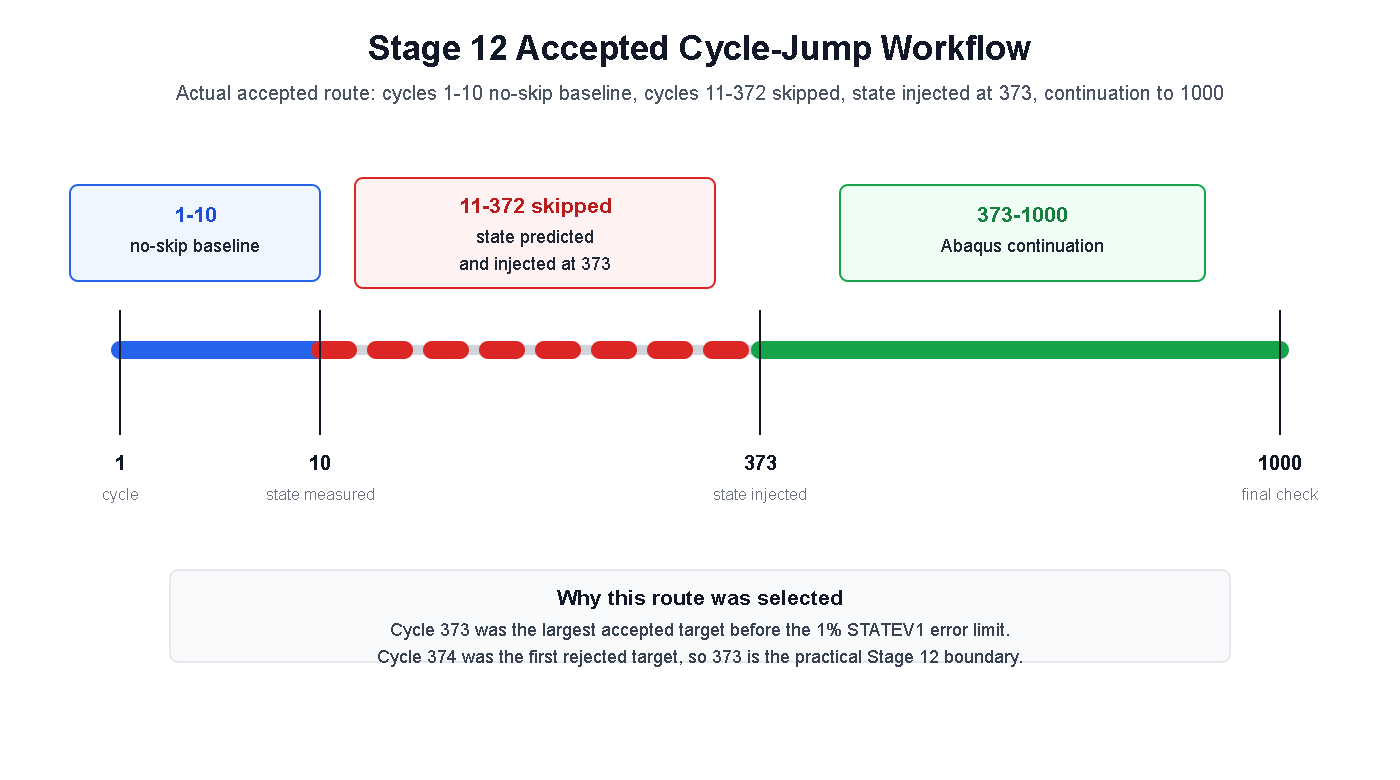
\includegraphics[width=0.92\linewidth]{fig04_stage12_accepted_workflow.png}
\caption{Latest accepted Stage 12 workflow: cycles 1--10 were solved cycle-by-cycle without skipping, the intermediate cycles 11--372 were skipped using the predicted state, and cycles 373--1000 were solved again in Abaqus after state reinjection.}
\end{figure}

\textbf{Explanation of Figure 7.}
The blue part means that Abaqus/Standard was run normally from cycle 1 to cycle 10, cycle-by-cycle without skipping. These cycles were used as the baseline window because the increment of \texttt{STATEV1} became nearly constant after the first few cycles. The red dashed part means that the intermediate cycles 11--372 were not solved by Abaqus; instead, the material state at cycle 373 was predicted from the measured cycle increment. The green part means that Abaqus was restarted from the injected state at cycle 373 and then continued normally to cycle 1000. Therefore this was not a direct jump from 10 to 1000. It was a jump from the measured cycle-10 state to the predicted cycle-373 state, followed by a real Abaqus continuation from 373 to 1000.

Cycle 373 was selected because it was the largest target cycle that still satisfied the 1\% final \texttt{STATEV1} error limit. Cycle 374 was the first target that exceeded the limit. This makes 373 the practical accepted boundary for the Stage 12 1000-cycle problem.

\begin{figure}[H]
\centering
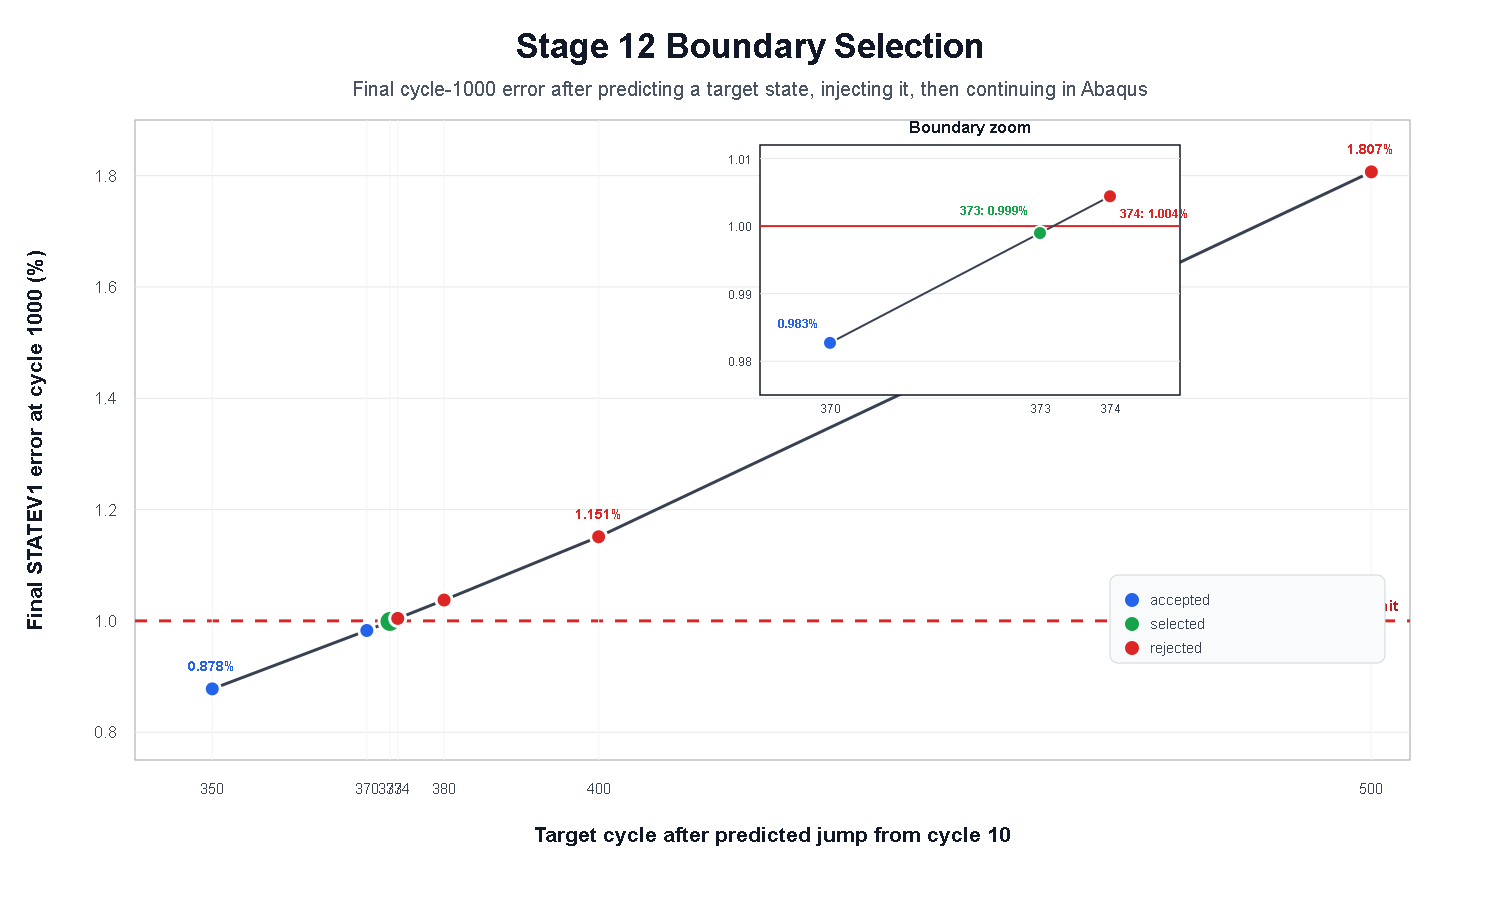
\includegraphics[width=0.92\linewidth]{fig05_stage12_boundary_selection.png}
\caption{Stage 12 target-cycle selection. The plotted value is the final \texttt{STATEV1} error at cycle 1000 after jumping from cycle 10 to the shown target cycle and then continuing in Abaqus.}
\end{figure}

\textbf{Explanation of Figure 8.}
The horizontal axis is the target cycle used for reinjection. For example, target 373 means: run cycles 1--10 cycle-by-cycle without skipping, skip the intermediate cycles 11--372, predict and inject the state for cycle 373, then let Abaqus solve cycles 373--1000. The vertical axis is the final percentage error of \texttt{STATEV1} at cycle 1000 compared with the full 1000-cycle no-skip reference simulation.

The blue points are accepted targets below the 1\% limit. The green point is the selected final route, target 373, with a final \texttt{STATEV1} error of 0.998969\%. The red points are rejected targets above the 1\% limit. Target 374 already gives 1.004410\% error, so it is just outside the acceptance rule. The conclusion is that the accepted Stage 12 workflow is:
\[
1\text{--}10\ \text{no-skip baseline}
\quad\rightarrow\quad
11\text{--}372\ \text{skipped; state injected at 373}
\quad\rightarrow\quad
373\text{--}1000\ \text{Abaqus continuation}.
\]

\begin{figure}[H]
\centering
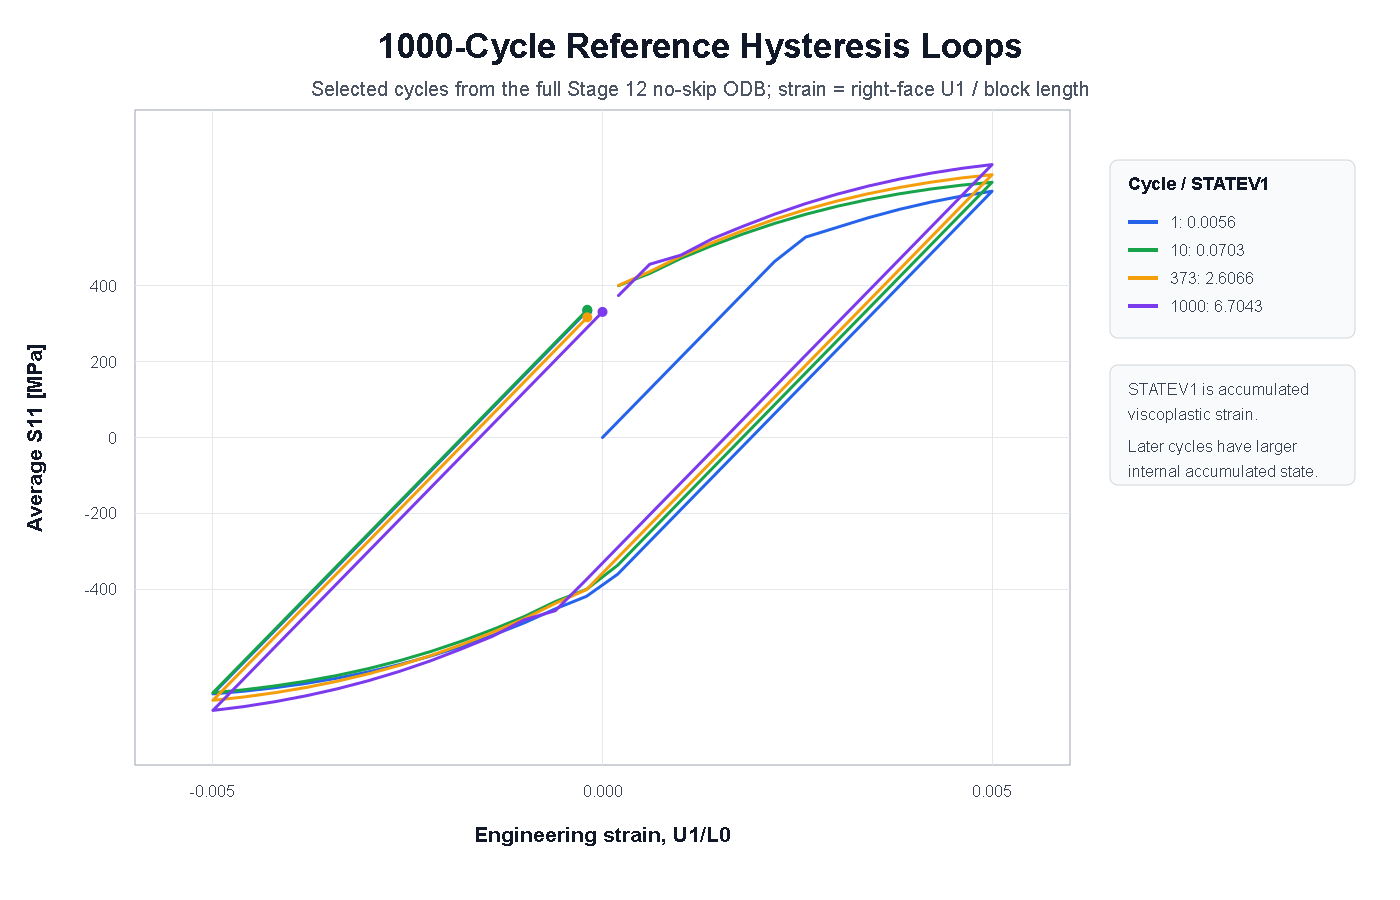
\includegraphics[width=0.92\linewidth]{fig06_stage12_1000cycle_hysteresis_statev1.png}
\caption{Selected hysteresis loops extracted from the full Stage 12 1000-cycle no-skip ODB. The plotted cycles are 1, 10, 373, and 1000, with the legend showing the corresponding \texttt{STATEV1} value.}
\end{figure}

\textbf{Explanation of Figure 9.}
This figure uses the full 1000-cycle reference ODB, not only the end-of-cycle CSV. The horizontal axis is engineering strain, computed from the average right-face displacement divided by the block length. The vertical axis is the average axial stress \texttt{S11}. Each colored loop is one selected cycle: cycle 1 shows the first transient response, cycle 10 is the baseline cycle used before prediction, cycle 373 is the accepted reinjection target, and cycle 1000 is the final reference cycle. The increasing \texttt{STATEV1} values in the legend show that accumulated viscoplastic strain grows over the simulation, even though the stress-strain loop shape remains bounded. This supports why \texttt{STATEV1} was used as the main long-cycle accuracy variable.

\section{UMAT Verification Before Cycle-Jump Use}

The UMAT was not treated as a black box. It was first checked on a simple single-element model before being used for cycle-jump validation.

The verification sequence was:

\begin{itemize}
  \item a one-element monotonic tension/compression smoke test to confirm compilation, linking, elastic response, and onset of inelastic evolution;
  \item a strain-controlled cyclic test at the selected $\pm0.5\%$ amplitude;
  \item an amplitude sweep to check that larger imposed strain amplitudes produced wider hysteresis loops and stronger accumulated viscoplastic strain;
  \item inspection of \texttt{STATEV1}, stress, displacement, and reaction-force trends before applying any cycle jump.
\end{itemize}

These checks do not prove that the UMAT is universally correct for every load path. They do show that, for the single-element cyclic validation problem used here, the UMAT gives the expected elastic/plastic/viscoplastic behavior before it is used in the cycle-jump workflow.

\section{UMAT Used}

The active UMAT is:

\begin{verbatim}
runs/chaboche_umat/umat/chaboche_vp_v1_working.f
\end{verbatim}

It is a simplified Chaboche-type unified viscoplastic UMAT. It includes:

\begin{itemize}
  \item isotropic elasticity;
  \item von Mises overstress;
  \item isotropic hardening;
  \item nonlinear kinematic hardening through backstress components;
  \item Perzyna-type rate dependence;
  \item 15 solution-dependent state variables.
\end{itemize}

The most important state variables are listed below. In Abaqus, \texttt{STATEV} means ``solution-dependent state variables.'' These are the internal memory variables that the UMAT stores at each integration point. They are not ordinary nodal displacements; they are material history quantities.

\begin{center}
\begin{tabular}{p{0.20\linewidth}p{0.70\linewidth}}
\toprule
\texttt{STATEV} index & Meaning \\
\midrule
1 & Accumulated viscoplastic strain, usually denoted $p$. This is the main scalar measure of irreversible cyclic deformation and was the controlling cycle-jump error variable. \\
2--7 & Backstress tensor components $X_{11}$, $X_{22}$, $X_{33}$, $X_{12}$, $X_{13}$, $X_{23}$. These store kinematic hardening, i.e. the translation of the yield surface during cyclic loading. \\
8--13 & Viscoplastic strain tensor components $\varepsilon^{vp}_{11}$, $\varepsilon^{vp}_{22}$, $\varepsilon^{vp}_{33}$, $\varepsilon^{vp}_{12}$, $\varepsilon^{vp}_{13}$, $\varepsilon^{vp}_{23}$. These store the irreversible strain state. \\
14 & Isotropic hardening stress $R_{iso}$. In this UMAT it can be recomputed from \texttt{STATEV1} and the material constants, but it is still written for output consistency. \\
15 & Last viscoplastic multiplier increment $\Delta p$. This is mainly a diagnostic value for the last increment, not a long-term independent history variable. \\
\bottomrule
\end{tabular}
\end{center}

When the report says that the later workflow injected all 15 \texttt{STATEV} values plus stress, it means that the continuation job was not initialized only with accumulated plastic strain. It also carried over the backstress, viscoplastic strain tensor, hardening output variables, and the stress tensor. This is closer to the real material state required for a physically meaningful Abaqus continuation.

The stress terms used in the report are:

\begin{center}
\begin{tabular}{p{0.22\linewidth}p{0.68\linewidth}}
\toprule
Term & Meaning \\
\midrule
S11 & Normal stress in the loading direction. This is the main stress component checked in the single-element test. \\
RF1 & Reaction force in direction 1, summed over the right-face node set. It checks whether the global force response is correct. \\
\texttt{RIGHT\_FACE} & Abaqus node set on the loaded face where displacement and reaction force were measured. \\
\texttt{U1} & Displacement in direction 1. In these continuation jobs the selected restart phase had right-face average \texttt{U1} near zero. \\
\bottomrule
\end{tabular}
\end{center}

No open-source URL or license header was found inside the local UMAT file. Therefore it should be described as a local/custom research UMAT rather than a confirmed open-source UMAT.

\section{Abaqus Data Extraction Map}

The table below states where each validation quantity came from. This is important because material history variables and stresses are integration-point quantities, while displacements and reaction forces are nodal quantities.

\begin{center}
\begin{tabular}{p{0.18\linewidth}p{0.22\linewidth}p{0.20\linewidth}p{0.16\linewidth}p{0.16\linewidth}}
\toprule
Quantity & Abaqus output & Position & Type & Use \\
\midrule
\texttt{STATEV1--STATEV15} & \texttt{SDV}/\texttt{STATEV} & integration point & material history & cycle-jump prediction and validation \\
\texttt{S11--S23} & \texttt{S} & integration point & stress tensor & stress reinjection through \texttt{SIGINI} \\
\texttt{U1} & \texttt{U} & right-face nodes & nodal displacement & strain/loading phase check \\
\texttt{RF1} & \texttt{RF} & right-face nodes & nodal reaction force & global force validation \\
Average \texttt{S11} & \texttt{S11} averaged over element/integration-point output & element/integration point & stress response & hysteresis loop \\
\bottomrule
\end{tabular}
\end{center}

\section{State Transfer: SDVINI and SIGINI}

To restart from a jumped material state, Abaqus must begin with the correct internal variables and stress. Two user subroutines were used:

\begin{itemize}
  \item \texttt{SDVINI}: initializes solution-dependent state variables;
  \item \texttt{SIGINI}: initializes stress.
\end{itemize}

The input deck must activate:

\begin{verbatim}
*INITIAL CONDITIONS, TYPE=SOLUTION, USER
*INITIAL CONDITIONS, TYPE=STRESS, USER
\end{verbatim}

This was not assumed. It was verified numerically at the first output frame.

\subsection{How the Starting State Was Verified}

The first-frame output was compared with the expected injected values. For the exact cycle-19 to cycle-20 state:

\begin{center}
\begin{tabular}{lll}
\toprule
Quantity & Expected injected value & First-frame evidence \\
\midrule
\texttt{STATEV1} & 0.13485494256 & matched exactly within tolerance \\
S11 & 335.576873779 MPa & matched exactly within tolerance \\
\bottomrule
\end{tabular}
\end{center}

For the predicted cycle-19 to cycle-20 jump:

\begin{center}
\begin{tabular}{ll}
\toprule
Check & Error \\
\midrule
First-frame \texttt{STATEV1} error & $5.12176806522\times10^{-9}$ \\
First-frame S11 error & $9.37347977015\times10^{-11}$ MPa \\
\bottomrule
\end{tabular}
\end{center}

This proves that the continuation simulation started from the intended state rather than from a fresh material state.

For the current single-element displacement-controlled validation, the injected state is considered numerically consistent if the first-frame \texttt{STATEV} values and stress match the intended values and the continuation proceeds without a sudden nonphysical jump in stress, reaction force, displacement phase, or convergence behavior. This is deliberately a single-element validation statement, not a general claim of full structural equilibrium for arbitrary geometries.

The reinjection proof therefore has four parts:

\begin{itemize}
  \item injected \texttt{STATEV} values compared with first-frame \texttt{STATEV} values;
  \item injected stress tensor compared with first-frame stress tensor;
  \item right-face displacement and reaction force checked at the first frame;
  \item continuation checked for artificial transients or convergence problems immediately after restart.
\end{itemize}

\section{What About the Displacement Field?}

The displacement field was not copied from a previous ODB as a full-field initial displacement. Instead, the continuation model was displacement-controlled and started at the intended load phase. In this simple single-element problem, that is acceptable because:

\begin{itemize}
  \item the deformation field is simple;
  \item the boundary displacement defines the continuation phase;
  \item the path memory is stored in \texttt{STATEV} and stress;
  \item first-frame stress and state-variable checks confirm the mechanical starting state.
\end{itemize}

For a larger structure, this would need more care. A general structural restart should also ensure compatibility of the displacement/strain field. The present work is a controlled single-element validation of the material-state reinjection method.

\section{Difference from the Nesnas-Saanouni Method}

The relevant reference is:

\begin{quote}
K. Nesnas and K. Saanouni, ``A cycle jumping scheme for numerical integration of coupled damage and viscoplastic models for cyclic loading paths,'' Revue Europeenne des Elements Finis, 9(8), 865--891, 2000. DOI: \url{https://doi.org/10.1080/12506559.2000.10511493}
\end{quote}

\subsection{Core Idea in the Nesnas-Saanouni Method}

Nesnas and Saanouni propose a two-time-scale integration method for coupled viscoplastic-damage cyclic problems. The fast scale is the usual time inside one loading cycle, and the slow scale is the cycle number. If the material state is written as
\[
\mathbf{Y}
=
\left[
\boldsymbol{\sigma},
\boldsymbol{\varepsilon}^{vp},
\mathbf{X},
R,
D,
\ldots
\right],
\]
where $\boldsymbol{\sigma}$ is stress, $\boldsymbol{\varepsilon}^{vp}$ is viscoplastic strain, $\mathbf{X}$ is kinematic hardening/backstress, $R$ is isotropic hardening, and $D$ is damage, the constitutive evolution can be written in rate form as
\[
\dot{\mathbf{Y}}=\mathbf{F}\left(\mathbf{Y},\boldsymbol{\varepsilon},T\right).
\]
Inside a cycle, they integrate this equation with an implicit constitutive algorithm:
\[
\mathbf{Y}_{N+1}
=
\Phi_{\mathrm{cycle}}\left(\mathbf{Y}_{N}\right),
\]
where $\Phi_{\mathrm{cycle}}$ is the result of solving one complete cycle. Across many cycles, they estimate the cycle derivative:
\[
\frac{d\mathbf{Z}}{dN}
\approx
\mathbf{Z}_{N+1}-\mathbf{Z}_{N},
\]
for a reduced set of stored variables $\mathbf{Z}$. A cycle jump of $\Delta N$ cycles is then made explicitly:
\[
\mathbf{Z}_{N+\Delta N}^{\mathrm{pred}}
=
\mathbf{Z}_{N}
+
\Delta N
\left(\frac{d\mathbf{Z}}{dN}\right)_{N}.
\]
The important point is that their method is a constitutive integration framework: it is designed to advance coupled viscoplastic and damage variables efficiently through cycle space while restoring enough internal variables to continue the simulation.

\subsection{Cycle-Jump Technique Used in This Work}

This thesis uses the same broad idea of separating fast within-cycle response from slow cycle-scale evolution, but the implementation is different and more practical for Abaqus/UMAT validation. Here, "cycle-by-cycle" or "no-skip" means Abaqus/Standard static cyclic analysis without cycle jumping; it does not mean Abaqus/Explicit. The main monitored variable is
\[
p = \texttt{STATEV1},
\]
the accumulated viscoplastic strain. From the no-skip baseline cycles, the stabilized per-cycle increment is computed as
\[
\overline{\Delta p}_{2-10}
=
\frac{1}{9}
\sum_{i=2}^{10}
\left(p_i-p_{i-1}\right).
\]
The scalar prediction from cycle 10 to a target cycle $N$ is then
\[
p_N^{\mathrm{pred}}
=
p_{10}
+
\left(N-10\right)\overline{\Delta p}_{2-10}.
\]

For the later reinjection stages, the same idea was extended from one scalar to a vector of injected state quantities:
\[
\mathbf{Q}
=
\left[
\texttt{STATEV1},\ldots,\texttt{STATEV15},
S_{11},S_{22},S_{33},S_{12},S_{13},S_{23}
\right].
\]
The later workflow does not extrapolate only \texttt{STATEV1}. It extrapolates and injects all 15 state variables and the six stress components. \texttt{STATEV} values are inserted through \texttt{SDVINI}, and stresses are inserted through \texttt{SIGINI}.

The vector prediction is
\[
\mathbf{Q}_{N}^{\mathrm{pred}}
=
\mathbf{Q}_{10}
+
\left(N-10\right)
\overline{\Delta\mathbf{Q}}_{2-10},
\]
with
\[
\overline{\Delta\mathbf{Q}}_{2-10}
=
\frac{1}{9}
\sum_{i=2}^{10}
\left(\mathbf{Q}_{i}-\mathbf{Q}_{i-1}\right).
\]
The predicted internal variables were inserted with \texttt{SDVINI}:
\[
\texttt{STATEV}_k(t_0)
=
\texttt{STATEV}_{k,N}^{\mathrm{pred}},
\qquad k=1,\ldots,15,
\]
and the predicted stress state was inserted with \texttt{SIGINI}:
\[
\boldsymbol{\sigma}(t_0)
=
\boldsymbol{\sigma}_{N}^{\mathrm{pred}}.
\]
The displacement field was not copied from an old ODB. Instead, the continuation model was restarted at the correct load phase using the prescribed boundary displacement. For the single-element validation model, the displacement phase is controlled directly by
\[
U_1(t_0)=U_{\max}A(t_0),
\]
where $A(t)$ is the cyclic amplitude function. This is acceptable for the present one-element material validation because the deformation field is simple and the path memory is mainly carried by \texttt{STATEV} and stress. For a larger structure, the displacement and strain fields would also need a stricter restart or mapping procedure.

\subsection{Acceptance Formula}

Every jump was checked against a full no-skip Abaqus reference. For any output quantity $q$, the percentage error was computed as
\[
e_q
=
\frac{
\left|q_{\mathrm{jump}}-q_{\mathrm{full}}\right|
}{
\max\left(\left|q_{\mathrm{full}}\right|,\epsilon\right)
}
\times100\%,
\]
where $\epsilon$ is a small number used only to avoid division by zero. For Stage 12, a clean accepted result required:
\[
e_{\texttt{STATEV1}}\leq1\%,
\qquad
e_{S11}\leq1\%,
\qquad
e_{RF1}\leq1\%.
\]
The limiting metric was \texttt{STATEV1}. Target cycle 373 gave
\[
e_{\texttt{STATEV1}}=0.998969\%,
\]
while target cycle 374 gave
\[
e_{\texttt{STATEV1}}=1.004410\%.
\]
Therefore, the accepted Stage 12 cycle-jump route was:
\[
1\text{--}10
\;\text{no-skip baseline}
\quad\rightarrow\quad
11\text{--}372
\;\text{skipped, state injected at 373}
\quad\rightarrow\quad
373\text{--}1000
\;\text{Abaqus continuation}.
\]

\begin{longtable}{p{0.24\linewidth}p{0.34\linewidth}p{0.34\linewidth}}
\toprule
Topic & Nesnas-Saanouni & This work \\
\midrule
\endhead
Purpose & General cycle-jump integration for coupled viscoplastic-damage models. & Practical Abaqus/UMAT implementation and validation. \\
Time scales & Uses an implicit within-cycle integration and an explicit large-cycle integration. & Uses no-skip Abaqus/Standard baseline cycles, cycle-space extrapolation, then Abaqus continuation after reinjection. \\
Jump formula & Advances a reduced set $\mathbf{Z}$ through cycle space using $\mathbf{Z}_{N+\Delta N}^{\mathrm{pred}}=\mathbf{Z}_N+\Delta N(d\mathbf{Z}/dN)_N$. & Uses $p_N^{\mathrm{pred}}=p_{10}+(N-10)\overline{\Delta p}_{2-10}$ and later the vector form $\mathbf{Q}_N^{\mathrm{pred}}=\mathbf{Q}_{10}+(N-10)\overline{\Delta\mathbf{Q}}_{2-10}$. \\
State variables & Restores a sufficient reduced set of evolving state variables for coupled models. & Started with scalar \texttt{STATEV1}; later injected all 15 \texttt{STATEV} values plus six stress components. \\
Damage & Includes coupled damage-viscoplasticity and is intended for fatigue damage analysis. & No damage variable in the current UMAT; the focus is accumulated viscoplastic strain and restart consistency. \\
Implementation & Constitutive algorithm with small-time and large-cycle scales. & External Python/PowerShell/Bash workflow around Abaqus, \texttt{SDVINI}, \texttt{SIGINI}, and UMAT. \\
Restart state & Restores selected internal variables inside the constitutive-cycle-jump framework. & Explicitly checks first-frame \texttt{STATEV1} and stress after reinjection to prove that the continuation starts from the intended state. \\
Validation & Gauss-point and structural examples. & No-skip Abaqus references at 20, 50, 100, 500, and 1000 cycles; Stage 12 accepted target 373 and rejected target 374. \\
\bottomrule
\end{longtable}

In short: Nesnas-Saanouni is the broader theoretical framework for integrating coupled viscoplastic-damage equations efficiently over many cycles. This work is a staged Abaqus implementation showing that predicted material states can be injected, verified, and used to skip cycles in a Chaboche UMAT problem. The main novelty in this thesis workflow is not a new constitutive theory, but the practical verification chain: no-skip baseline cycles, state prediction, \texttt{SDVINI}/\texttt{SIGINI} reinjection, first-frame state check, continuation analysis, and comparison with full no-skip reference simulations.

\section{Long-Cycle Evolution and Justification for Cycle Jumping}

The professor's main long-cycle question is whether the slow variable stabilizes or keeps drifting. A complete Stage 14 blockwise comparison is still pending, but the salvaged Stage 13 partial no-skip reference provides a useful diagnostic history through cycle 4380. This partial reference came from the 5000-cycle HPC job that stopped at the teaching-queue walltime limit, so it is not used as a final 5000-cycle validation reference. It is used here only to study long-cycle trends.

\begin{figure}[H]
\centering
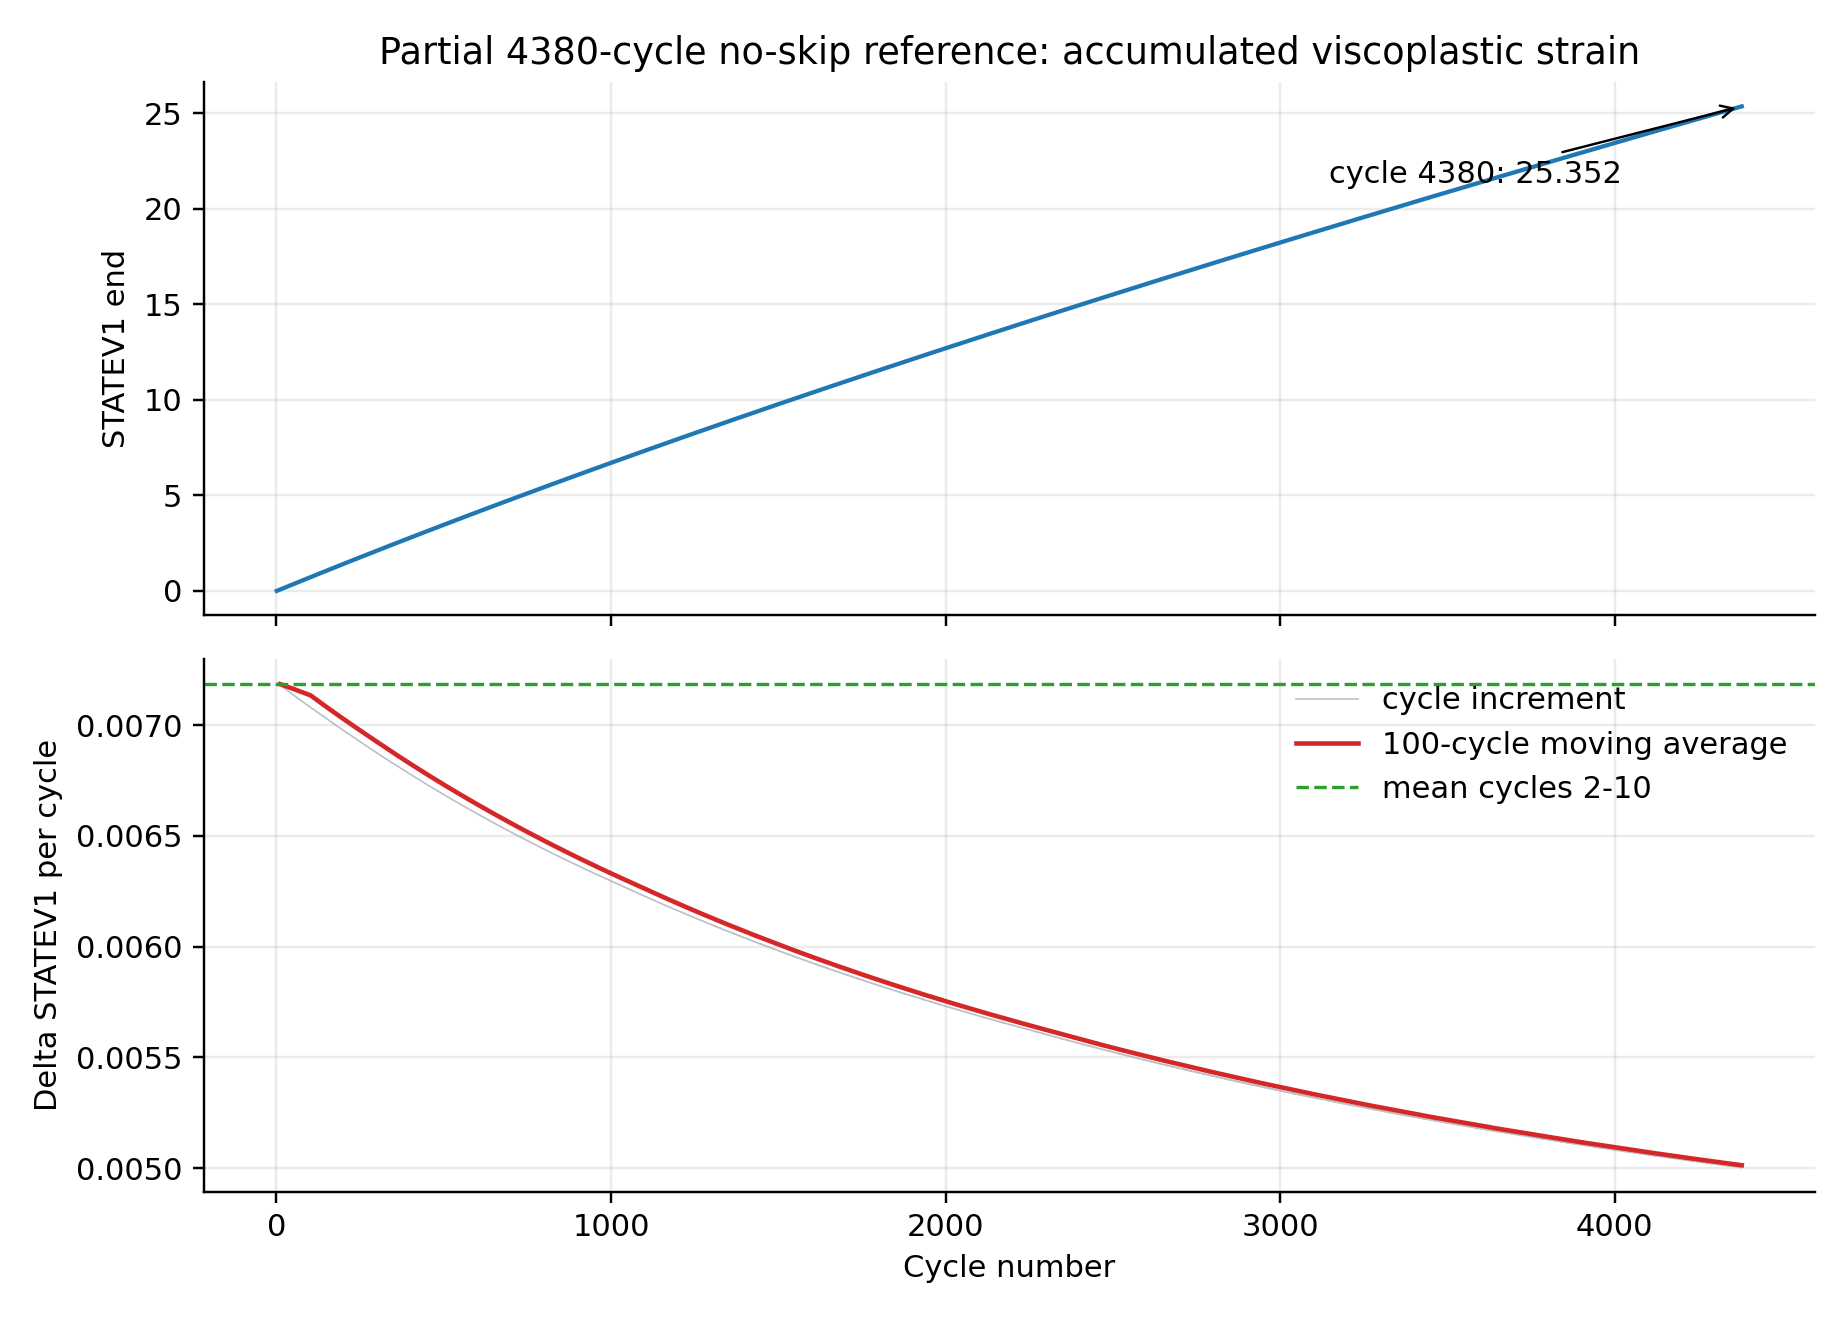
\includegraphics[width=0.92\linewidth]{fig07_stage13p_4380_statev1_delta.png}
\caption{Long-cycle evolution from the partial 4380-cycle no-skip reference. \texttt{STATEV1} continues to increase, while the per-cycle increment decreases gradually.}
\end{figure}

\begin{figure}[H]
\centering
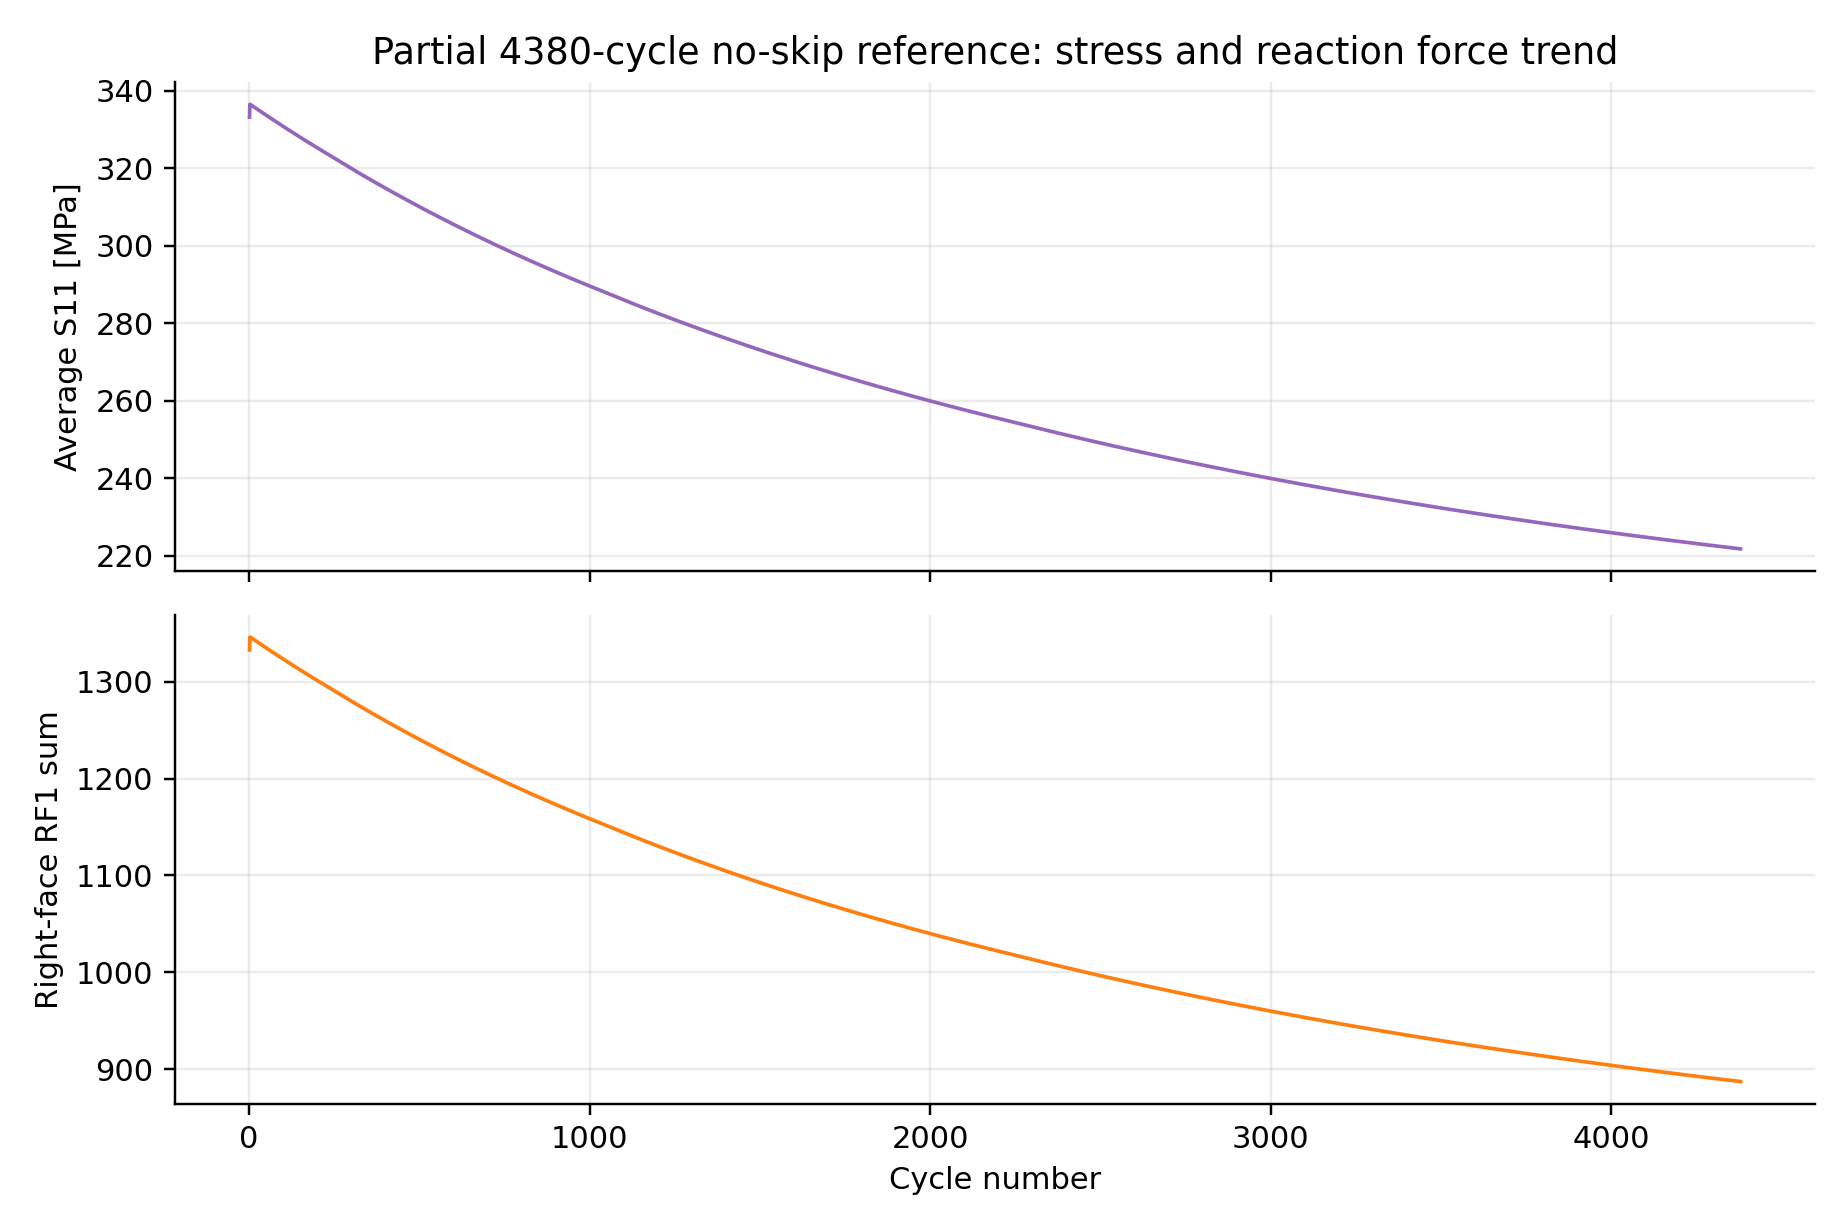
\includegraphics[width=0.92\linewidth]{fig08_stage13p_4380_s11_rf1.png}
\caption{Average \texttt{S11} and summed right-face \texttt{RF1} from the same partial 4380-cycle no-skip reference. These quantities evolve slowly with cycle number and remain bounded.}
\end{figure}

\begin{center}
\begin{tabular}{lr}
\toprule
Diagnostic quantity & Value \\
\midrule
\texttt{STATEV1} at cycle 10 & 0.0702667832375 \\
\texttt{STATEV1} at cycle 1000 & 6.70427989960 \\
\texttt{STATEV1} at cycle 2000 & 12.6968250275 \\
\texttt{STATEV1} at cycle 4380 & 25.3516654968 \\
Mean $\Delta\texttt{STATEV1}$, cycles 2--10 & 0.00718546519056 \\
Mean $\Delta\texttt{STATEV1}$, cycles 1000--2000 & 0.00599284891363 \\
Mean $\Delta\texttt{STATEV1}$, cycles 3000--4380 & 0.00516311540541 \\
\bottomrule
\end{tabular}
\end{center}

The conclusion is mixed but useful. \texttt{STATEV1} does not stabilize to a flat constant by cycle 4380; it keeps increasing, so long-cycle acceleration remains meaningful. However, the increment is not perfectly constant. The early cycles 2--10 slope is higher than the late-cycle average, so a single long linear extrapolation from the first 10 cycles tends to overpredict later accumulated viscoplastic strain. This is consistent with the Stage 12 boundary result: cycle jumping is useful, but it must be bounded and re-anchored against no-skip reference data.

The partial 4380-cycle trend shows that the early cycles 2--10 slope is not globally valid for very long extrapolation. Therefore, the next logical step is not one larger jump, but a blockwise cycle-jump strategy where the slope is periodically re-estimated from newer no-skip or continuation data.

For the completed 1000-cycle validation, the maximum accepted target was cycle 373, corresponding to the route cycle 10 $\rightarrow$ predicted cycle 373 $\rightarrow$ Abaqus continuation to cycle 1000. Target cycle 374 was the first rejected case under the 1\% \texttt{STATEV1} criterion. The longer partial trend supports the need for Stage 14 blockwise jumping: repeated shorter jumps with updated slopes are more defensible than one very long extrapolation from cycles 2--10.

\section{Professor-Feedback Response Table}

\begin{longtable}{p{0.25\linewidth}p{0.40\linewidth}p{0.25\linewidth}}
\toprule
Professor question & Response / evidence & Remaining work \\
\midrule
\endhead
How do you know the UMAT is correct? & Single-element monotonic and cyclic checks were performed before cycle-jump use. The UMAT produced reasonable elastic/plastic/viscoplastic behavior and amplitude-dependent hysteresis. & Add a more formal analytical or simple benchmark comparison. \\
Which slope did you use? & Mean cycle-by-cycle increment from cycles 2--10, not a single secant between cycle 2 and cycle 10. & Cite the exact CSV/source table beside the formula. \\
What data did you extract? & \texttt{STATEV}/\texttt{S} from integration-point output; \texttt{U}/\texttt{RF} from right-face nodes. & Keep the extraction map in the final thesis chapter. \\
Is the injected state correct? & First-frame \texttt{STATEV1} and stress match the injected values within numerical tolerance; continuation proceeds from the intended load phase. & Add a compact RF/transient table for each accepted jump. \\
Did you inject stress? & Later stages inject all 15 \texttt{STATEV} values plus six stress components. \texttt{STATEV} uses \texttt{SDVINI}; stress uses \texttt{SIGINI}. & Keep this visible in the method section. \\
Is cycle jumping necessary? & The 1000-cycle result and partial 4380-cycle trend show \texttt{STATEV1} still evolves; it has not flattened by cycle 4380. & Finish/confirm Stage 14 blockwise results when HPC access is available. \\
Is linear extrapolation valid? & Valid only inside the accepted jump boundary. Stage 12 accepted target 373 and rejected target 374 under the 1\% \texttt{STATEV1} limit. & Compare blockwise slopes in Stage 14 instead of relying on one early slope. \\
\bottomrule
\end{longtable}

\section{Completed Simulation Milestones}

\begin{longtable}{p{0.25\linewidth}p{0.21\linewidth}p{0.45\linewidth}}
\toprule
Stage / case & Status & Main result \\
\midrule
\endhead
1-cycle UMAT smoke test & completed & UMAT compiled, linked, and ran in Abaqus. \\
10-cycle baseline & completed & Stable \texttt{Delta STATEV1}; mean cycles 2--10 = 0.007185465191. \\
20-cycle validation & completed & Predicted cycle-20 \texttt{STATEV1} error = 0.049427232695\%. \\
50-cycle reference & completed & Used as reference for cycle-28, 30, 40, and 50 checks. \\
Stage 4 exact-state injection & completed & \texttt{SDVINI} and \texttt{SIGINI} reproduced starting state at first frame. \\
Stage 5B predicted 19 to 20 & accepted & \texttt{STATEV1} error = 0.049427232695\%; S11 error = 0.127012627651\%. \\
Stage 6D predicted 29 to 30 & exploratory success & \texttt{STATEV1} error = 0.0458269043313\%; S11 error = 2.34365652874\%. \\
Stage 7C predicted 27 to 28 & exploratory success & \texttt{STATEV1} error = 0.0231584782019\%. \\
Stage 9B predicted 49 to 50 & accepted & Skipped 38 intermediate FE cycles; \texttt{STATEV1} error = 0.253071065812\%. \\
Stage 10B predicted 99 to 100 & accepted & Skipped 88 intermediate FE cycles; \texttt{STATEV1} error = 0.667869616047\%. \\
Stage 11H accepted boundary refinement & accepted exploratory & Cycle 10 $\rightarrow$ predicted cycle 141 $\rightarrow$ cycle 142; skipped 130 intermediate FE cycles; final \texttt{STATEV1} error = 0.999121505495\%. \\
Stage 11B aggressive 500-cycle stress test & completed but rejected & Deliberate over-jump from predicted cycle 499 to cycle 500; stable run, but final \texttt{STATEV1} error = 3.69823703261\%. \\
Stage 12 target 373 to 1000 & accepted & Skipped 362 intermediate FE cycles; final \texttt{STATEV1} error = 0.998969124476\%. \\
Stage 13 partial 4380-cycle reference & diagnostic only & \texttt{STATEV1} still increased to 25.3516654968 by cycle 4380; late-cycle increment was lower than the cycles 2--10 slope. \\
\bottomrule
\end{longtable}

\textbf{Excluded from accepted cycle-jump results:} the partial 4380-cycle Stage 13 work and the current Stage 14 2000-cycle blockwise work. Stage 13 partial data is included only as long-cycle diagnostic evidence.

\section{Final Takeaway}

The project has moved from a simple scalar cycle-jump idea to a verified Abaqus/UMAT reinjection workflow. The strongest evidence is that the injected state appears correctly in the first frame, and accepted long-horizon jumps remain below the 1\% accumulated-state error threshold. For the 1000-cycle Stage 12 problem, the current practical accepted target is cycle 373, i.e. 37.3\% of the total cycle count; target 374 was the first rejected case.

\end{document}
